
\documentclass[natbib,referee]{svjour3}

\smartqed  % flush right qed marks, e.g. at end of proof


% PACKAGES
% ------------------------------------------------------------------------------

\usepackage{simplemargins}
\usepackage{textcomp}
\usepackage{amsbsy}
\usepackage[dvipsnames]{xcolor}

\usepackage{graphicx}
\usepackage[pdftex,bookmarks=false]{hyperref}
\usepackage{float}
 \usepackage{multirow}

% LINKS
% ------------------------------------------------------------------------------

\hypersetup{
    pdfpagelayout=OneColumn,
    colorlinks = true,
    urlcolor   = blue,
    citecolor  = blue,
    linkcolor  = blue
}
\urlstyle{same}


% ADDITIONAL COMMANDS
% ------------------------------------------------------------------------------

\newcommand{\myrevision}[1]{\textcolor{Black}{#1}}
\settopmargin{1.2in}
\setleftmargin{.9in}
\setrightmargin{1in}
\setbottommargin{.2in}


% JOURNAL NAME
% ------------------------------------------------------------------------------

\journalname{Not Decided}


% MAIN DOCUMENT STARTS
% ==============================================================================


\newcommand{\vsmin}{$V_{S_{\min}}$}
\newcommand{\vsmineq}[1]{$V_{S_{\min}}=#1$~m/s}
\newcommand{\vsthirty}{$V_{S30}$}
\newcommand{\vs}{$V_{S}$}
\newcommand{\vseq}[1]{$V_{S}=#1$~m/s}

\newcommand{\vp}{$V_{P}$}
\newcommand{\vpeq}[1]{$V_{P}=#1$~m/s}

\newcommand{\qp}{$Q_{P}$}
\newcommand{\qs}{$Q_{S}$}
\newcommand{\qk}{$Q_{K}$}
\newcommand{\qsvs}{$Q_{S}-V_{S}$}
\newcommand{\qpqs}{$Q_{P}-Q_{S}$}
\newcommand{\qsoqp}{$Q_{S}/Q_{p}$}

\newcommand{\feq}[1]{$f=#1$~Hz}
\newcommand{\fleq}[1]{$f\leq#1$~Hz}
\newcommand{\fgeq}[1]{$f\geq#1$~Hz}
\newcommand{\fmax}{$f_{_{\max}}$}
\newcommand{\fmaxeq}[1]{$f_{_{\max}}=#1$~Hz}

\newcommand{\eqmag}[1]{$M_{#1}$}

\newcommand{\adomain}[3]{#1~#3 $\times$ #2~#3}
\newcommand{\vdomain}[4]{#1~#4 $\times$ #2~#4 $\times$ #3~#4}

\begin{document}


% TITLE
% ------------------------------------------------------------------------------

\title{A Surrogate-based Optimization Approach for Calibration of Attenuation Models (\qsvs{} Relationships) Used in Physics-Based Ground-Motion Earthquake Simulation}
\titlerunning{\qsvs{} Relationships}


% AUTHORS
% ------------------------------------------------------------------------------

\author{%
    Naeem Khoshnevis \and 
    Ricardo Taborda
}

% \authorrunning{N.~Khosh} % if too long for running head

\institute{
    N. Khoshnevis
       \at
        Center for Earthquake Research and Information\\
        The University of Memphis, Memphis, TN 38152, U.S.A.\\
        \email{nkhshnvs@memphis.edu}\\
    R. Taborda 
        \at
        Center for Earthquake Research and Information\\
        and Department of Civil Engineering
        The University of Memphis, Memphis, TN 38152, U.S.A.
}

\date{Received: date / Accepted: date}

\maketitle

\begin{abstract}
    %
We present a customized solution approach to study attenuation models through combining machine learning, ground motion simulation, and optimization methods. The accurate solution of wave propagation problems requires the appropriate representation of energy losses due to internal friction in geomaterials. These losses are important because their mischaracterization may lead to the over- or under-estimation of the amplification and duration of seismic waves in regions with high dissipative properties. Recent studies show that synthetics from physics-based simulations tend to attenuate with distance at different rates than observations, thus suggesting that current approaches to modeling attenuation need to be revised. In physic-based ground-motion simulation, the attenuation of seismic waves is typically treated by means of viscoelastic models. Internally, the properties used for these models are set based on the material's quality factor Q. The value of Q for shear waves, Qs, for instance, is usually defined based on rules that depend on the value of the shear wave velocity, Vs.  Typical Qs-Vs relationships are (piecewise) linear or polynomial functions. Several Qs-Vs relationships exist in the literature. There is, however, no consensus about the most appropriate one. We propose new methodology based on  combining machine learning (artificial neural network) techniques and optimization methods to narrow and customize the search domain for each station in studying the Q factor parameters in physics-based ground motion simulation. First we train a neural network to predict the requested signal's parameters, using the trained network as a cost function in optimization process, we optimized the parameters for recorded data and compute several potential Q parameters. We use the mean Q as an actual target value and repeat the optimization process. This step provides the dominant shear wave velocity ranges. We return back to the original optimization results and choose the Q data that belong to dominant shear wave velocity range. We present successful applications of the proposed method on homogeneous, layered, and actual heterogenous domains. The proposed method shows how integration of emerging computational resources with machine learning techniques can improve anelastic attenuation models' optimization processes. Analysis of observational data, due to noise, potential rotation of stations during earthquake, mistakes in preprocessing data and many more other factors, mostly leave a user and optimization algorithm with a very large search domain. The proposed method, on the other hand,  provides potential search domain which is tailored with observational data. We applied the proposed model on several recorded data of  $Mw ~5.4$ 2008 Chino Hills earthquake and discuss the results. 




    \keywords{Anelastic Attenuation \and 
3D Ground Motion Simulation \and
Machine Learning \and
Surrogate-based Optimization
}
\end{abstract}



\section{Introduction}

The accurate solution of wave propagation problems requires the appropriate representation of energy losses due to internal friction in geomaterials. These losses are important because their mischaracterization may lead to the over- or under-estimation of the amplification and duration of seismic waves in regions with high dissipative properties. The amplitude of seismic waves decreases as the distance from source increases. In the absence of large deformations (i.e., nonlinearities), this is due to Geometric spreading, intrinsic attenuation, and scattering. Geometric spreading and scattering (as a result of heterogeneous velocity model) are inherently considered in $3D$ physics-based ground motion simulation. Intrinsic attenuation, on the other hand, is a result of irreversible changes in the crystal defect structures of the medium and should be considered in synthetic models. These media are called anelastic, and the configuration of material particles is to some extent dependent on the history of applied stress \citep{Aki_2002_Book}. Intrinsic attenuation or internal friction is studied by means of quality factor ($Q$), which is inversely related to the strength of the attenuation. From the definition of $Q$ (fractional energy loss per cycle), it is concluded that the rate of attenuation increases with frequency. Therefore, $Q$ is considered as a frequency-depended parameter \citep[e.g., see][ and references therein.]{Adams_1998_GJI, Mousavi_2014_JGR, Sedaghati_2015_BSSA, Nazemi_2017_TP} Specifically at \fgeq{1} \citep[e.g., see ][]{Withers_2015_BSSA}. High-frequency $Q$ can be dependent on numerous factors. \citet{Hauksson_2006_JGR} showed that $Q$ could be different on a regional scale due to local impedance contrasts, chemical composition, crack structure, grain boundary movement, crustal fluids, and, to a lesser extent, temperature variations within the brittle seismogenic crust. At lower frequencies (\fleq{1}), given the wavelengths and minimum velocities of physics-based ground motion simulation, $Q$ is considered as a function of shear wave velocity (\vs{}) and its frequency and depth dependency has been ignored.\\
In physics-based earthquake ground-motion simulation, the attenuation of seismic waves is typically treated by means of viscoelastic models \citep[e.g.,][]{Day_2001_BSSA, Graves_2003_BSSA, Kaser_2007_GJI, Bielak_2011_G}. These models are made of mechanisms that employ numerical techniques to account for the dissipative and transient characteristics of the ground motion. Internally, the properties of a given attenuation model are set based on the material's $Q$. Community velocity models ($CVMs$) used in simulations do not generally provide values of $Q$. Instead, the most common approach is to define the quality factors associated with $P$ and $S$ waves, \qp{} and \qs{}, based on the values of the seismic velocities \vp{} and \vs{} obtained from any particular $CVM$.\\
Several  \qsvs{} relationships exist in the literature. There is, however, no consensus about the most appropriate one. To the best of our knowledge, none of these studies have undertaken a comprehensive search for optimal $Q$ model. For example, \citet{Olsen_2003_BSSA} constructed several simple distributions of  \qs{} and \qp{} and identified those that provide the best fit between simulated and recorded $0-0.5~Hz$ peak velocities for the 1994 Northridge earthquake. Although their suggested models significantly improved the goodness-of-fit between synthetic and observation, the lack of consensus among different studies suggests the idea that a comprehensive search for optimal $Q$ should be considered. In this paper, we propose to use a parametric \qsvs{} relationship and we present a surrogate-based optimization method to better constraining the parameters of models used to represent the effects of intrinsic attenuation. We set up a genetic algorithm (GA) optimization process as an evolutionary algorithm to search for the best \qsvs{} relationship parameters by minimizing a cost function.  Cost functions, in simple words, are the absolute difference between proposed parameters solution and target values. Optimization process needs to run ground motion simulation hundreds of thousands of times, whereas generating accurate ground motion simulation models are computationally expensive and time-consuming. Therefore, based on numerous simulation results, we develop surrogates (or meta-models) to estimate the target values based on arbitrary \qsvs{} relationship input parameters. Although previous studies use peak ground velocity (PGV) as a metric for estimating energy loss \citep[e.g., see ][{\color{red} needs more references.}]{Olsen_2003_BSSA}, our study shows using other metrics can increase the uniqueness of signals and consequently optimization process. Therefore, the surrogates, which are developed using artificial neural networks, trained to estimate PGV, peak ground acceleration (PGA), acceleration response spectra (SA), and area under velocity signal envelop (Venp). Complicated source model, complex geological features, and stations distance from source make the study process unique for each station. In this study, we address this issue through our proposed method. \\
In summary, through a sequence of an optimization process, we locate the most effective shear wave velocity range that a station and optimization process, most probably, are capable of estimating the \qsvs{}, accurately.  relationship values. Therefore, from each station, we only choose those data, if there is any, which we have higher confidence in its accuracy. We test the proposed method on homogenous, layered, and heterogeneous domains.  We discuss the application of the method on a comparison of simulations for $Mw~5.4$ 2008 Chino Hills earthquake (\vsmin$=350~$m/s and \fmax$=1$~Hz) as a heterogeneous domain and compare the results with previous studies. Application of the method on different domains shows that it is robust, and based on the simulation model, station location, and metrics that are used, it can confidently locate the $Q$ values. 































\section{Attenuation Models}

In physics-based ground motion simulation, $Q$ is considered as a user-defined value. Community velocity models ($CVMs$) used in simulations do not generally provide values of $Q$. Such a high resolution $Q$ model requires a rigorous inversion process. Therefore, the value of \qs{}, for instance, is usually defined based on rules that depend on the value of \vs{}. Typical forms of \qsvs{} relationships are (piecewise) linear or polynomial functions \citep[e.g.,][]{Brocher_2008_BSSA, Brocher_2005_Tech,Olsen_2003_BSSA, Graves_2008_BSSA,Taborda_2013_BSSA}. The value of \qp{} is mostly defined in terms of \qs{}, and, in some cases, also on the velocity contrast, $V_{P}/V_{S}$. Table~\ref{tab:QsVstable} shows a collection of different \qsvs{} and \qpqs{} relationships used in simulations and other related studies, including the earthquake or scenario event for which they were employed, and the simulation's minimum shear wave velocity (\vsmin{}) and maximum frequency (\fmax{}). Fig.~\ref{fig:Figure_q_models}  shows the \qs{} values with respect to \vs{} for each \qsvs{} relationship.  

% Please add the following required packages to your document preamble:
% \usepackage{multirow}
\begin{table}[]
	\centering
	\caption{Examples of \qsvs{} and \qpqs{} relationships used in past physics-base simulations}
	\label{tab:QsVstable}
	\renewcommand{\arraystretch}{0.75}
	\resizebox{\textwidth}{!}{%
		\begin{tabular}{lccccccc}
			\textbf{Publication}                                                        		    & \textbf{Simulation}                                       &  \textbf{\vsmin{}}             & \textbf{\fmax{}}                          & \multicolumn{3}{c}{\textbf{\qs{}=g(\vs{})}}                     &\textbf{\qp{}=h(\qs{})}                                 \\ 
			                                                                                       		    &                                                                     &  \textbf{(m/s)    }             & \textbf{(Hz)}                                 & \multicolumn{3}{c}{\textbf{($V_{S}$ in km/s, depth $z$ in km)}}         &                               \\ \hline
			\citet{Olsen_2003_BSSA}                                             		    & 1994 Northridge                                          & \multirow{2}{*}{500}        & \multirow{2}{*}{0.5}                    & 20\vs{}                                                             &   & \vs{}$< 1.5$                           & \multirow{2}{*}{1.5\qs{}} \\ 
			\citet{Olsen_2008_BSSA}                                              		    & TeraShake$$                                               &                                        &                                                   & 100\vs{}                                                           &   & \vs{} $\geq 1.5$                       &                            \\\hline
			\citet{Olsen_2009_GRL}                                               		    & ShakeOut                                                    & \multirow{3}{*}{500}        & \multirow{3}{*}{0.5}                    & \multicolumn{3}{c}{\multirow{4}{*}{50\vs{}}}     & \multirow{4}{*}{2\qs{}}                             \\
			\citet{Bielak_2010_GJI}$^{FD}$                                    		    &  ShakeOut                                                   &                                        &                                                   & \multicolumn{3}{c}{}                                          &                                                 \\
			\citet{Graves_2011_PAG}                                              		    & CyberShake                                                &                                         &                                                  & \multicolumn{3}{c}{}                                          &                                                 \\ \cline{3-4}
			\citet{Cui_2010_Proc}                                                   		    & M8                                                               & 400                                  & 2.0                                            & \multicolumn{3}{c}{}                                          &                                                 \\ \hline
			\multirow{2}{*}{\citet{Komatitsch_2004_BSSA}}             		    & 2001 Hollywood                                          & \multirow{2}{*}{670}         & \multirow{2}{*}{0.5}                   & 90                                 &   & Sediments                              & \multirow{2}{*}{$\infty$}  \\
			                                                                                        		    & 2002 Yorba Linda                                        &                                         &                                                  & $\infty$                           &   & Bedrock                                &                            \\ \hline
			\citet{Taborda_2006}$^\mathsection$                              		    & TeraShake                                                   & 300                                  & 1.0                                            & \multicolumn{3}{c}{\multirow{3}{*}{50\vs{}}}                                                                                  &                                                                 \\
			\citet{Taborda_2007} $^\mathsection$                            	            & ShakeOut                                                    & 200                                  & 1.0                                             & \multicolumn{3}{c}{}                                                                                                                    &                                                                  \\
			\citet{Bielak_2010_GJI}$^{FE,}$$^\mathsection$                            & ShakeOut                                                   & 500                                   & 0.5                                            & \multicolumn{3}{c}{}                                                                                                                    &                                                                 \\ \hline
			\citet{Graves_2008_BSSA}                                    		             & 2001 Big Bear                                            & 250                                   & 1.0                                            & \multicolumn{3}{c}{60\vs{}}                                                                                                           &                                                 \\ \cline{5-7}
			\multirow{3}{*}{\citet{Aagaard_2008_BSSA}}            			     & \multirow{3}{*}{1989 Loma Prieta}             & \multirow{3}{*}{330-760}   & \multirow{3}{*}{0.5-1.0}             & $50V_{S}$         &   & $V_{S}< 0.9$                           & \multirow{6}{*}{$2$\qs{}}  \\
			                                                                                    		  	     &                                                                    &                                         &                                                   & $60 V_{S}^{1.5}$                   &   & $0.9 \leq V_{S}<3.4$                   &                            \\
			                                                                                       		     &                                                                    &                                         &                                                  & $500$                              &   & $3.4 \geq V_{S}$                       &                            \\ \cline{5-7}
			\multirow{3}{*}{\citet{Brocher_2008_BSSA}$^\mathparagraph$}     &                                                                     &                                        &                                                   & 13                                 &   & $V_{S}<0.3$                            &                            \\
			                                                            					    &                                                                     &                                         &                                                   & $-16+104.13V_{S}$                  &   & \multirow{2}{*}{$0.3\leq V_{S} < 5.0$} &                            \\
			                                                            					    &                                                                     &                                         &                                                   & $-25.225{V_{S}}^2+8.2184{V_{S}}^3$ &   &                                        &                            \\ \hline
			\citet{Chaljub_2010_BSSA}$^\dagger$                                           & 2003 Lancey, and                                        & \multirow{2}{*}{300}        & \multirow{2}{*}{2.0}                     & 50                                 &   & $z<1$                                  & $3/4(V_{P}/V_{S})^2Q_{S}$  \\
			                                                            				            & Event S1                                                      &                                        &                                                    & $\infty$                           &   & $z\geq1$                               & $\infty$                   \\ \hline
			\citet{Taborda_2013_BSSA}                                    			    & \multirow{2}{*}{2008 Chino Hills}                 & \multirow{2}{*}{200}        & \multirow{2}{*}{4.0}                     & \multicolumn{3}{c}{\multirow{3}{*}{\begin{tabular}[c]{@{}c@{}}$10.5 - 16V_{S} + 153 V_{S}^2-103V_{S}^3$\\ $+ 34.7V_{S}^4-5.29*V_{S}^5+0.31V_{S}^6$\end{tabular}}} & \multirow{3}{*}{$3/4(V_{P}/V_{S})^2Q_{S}$} \\
			\citet{Taborda_2014_BSSA}                                    			    &                                                                     &                                        &                                                    & \multicolumn{3}{c}{}                                                                                                                        &                                                 \\ \cline{1-4}
			\citet{Taborda_2016_GJI}                                                                & 30 earthquakes                                           & 200                                  & 1.0                                              & \multicolumn{3}{c}{}                                                                                                                        &                                                 \\ \hline
			\citet{Withers_2015_BSSA}$^\ddagger$                                         & 2008 Chino Hills                                         & 200                                  & 4.0                                               & \multicolumn{3}{c}{$100V_{S}$}                                                                                                       & $2$\qs{}                                              \\ \hline
			\multicolumn{4}{l}{$*$ Denotes scenario events}                                                                                & \multicolumn{4}{l}{$\dagger$ Simulations for Grenoble Valley, France}                                                                                                                                                                                                                   \\
			\multicolumn{4}{l}{$\mathsection$ Rayleigh damping instead of a visco-elastic model}                     & \multicolumn{4}{l}{$^{FE}$ Finite-element simulation results therein}                                                                                                                                                                                                                 \\
			\multicolumn{4}{l}{$\mathparagraph$ Empirical relations (no simulation) for Northern California}     & \multicolumn{4}{l}{$^{FD}$ Finite-difference simulation results therein}            \\
			\multicolumn{4}{l}{$\ddagger$ Frequency independent part of $Q$}                                                  & \multicolumn{4}{l}{}                                                                                                                                                                                                     
		\end{tabular}}
\end{table}

 \begin{figure}
    \centering
    \includegraphics[width=400 px]{figures/pdf/Figure_01.pdf}
    \caption{Illustration of \qsvs{} relationships introduced in Table~\ref{tab:QsVstable}.}
    \label{fig:Figure_q_models}
\end{figure}

This figure illustrates the significant differences between these models. There is no consensus on the most appropriate set of relationships between seismic velocities and quality factors. The relationship used by \citet{Taborda_2013_BSSA} was introduced as an attempt to capture some of the main features of other \qsvs{} rules. It is known that the relationships between \qs{} and \vs{}, and between \qp{} and \qs{} can be depth dependent (see, for instance, \citet{Olsen_2003_BSSA}, and the references therein) although \qs{} remains strongly correlated with \vs{}.  \citet{Hauksson_2006_JGR} also show that while \qs{} and \qp{} increase rapidly with depth consistent with the crustal structure, but argue that the ratios between \qs{} and \qp{} vary with depth and are different within and outside the major basins in southern California. They obtained values of \qsoqp$>1$ for most of the region but found a few limited areas, mostly outside the major sedimentary basins, where \qsoqp$< 1$. \citet{Song_2013_AGU} concluded that, in general, $Q_{S} \geq Q_{P}$, with $Q_{S} \approx Q_{P}$ near the surface $(z < 5 km)$ but $Q_{S} > Q_{P}$ at depth; and indicated that \qs{} seems to be in better agreement with the rule $Q_{S} = 50V_{S}$ at depth but not near the surface, where \qs{} is not linearly related to \vs{}. However, most of the simulations done recently (as seen in Table.~\ref{tab:QsVstable}) correspond to numerical models with maximum frequencies, \fmax{} $\leq1-2$~Hz, and minimum shear wave velocities, \vsmin{}$\geq300$~ m/s, where one can still assume $Q$ to be frequency independent. 







\section{Methodology}

The objective of this paper is to present a method based on combination of machine learning and optimization process in order to narrow the search domain and customize solution for each station. Earthquakes are recorded in different stations; and our knowledge and understanding of seismic parameters are mostly based on these recorded data. In physics-based ground motion simulation specially at low frequencies, peak ground velocity of S wave arrivals is the most common indicator of energy loss \citep[e.g., see][]{olsen2003estimation}. It is a common practice to include all stations results to develop the final model. However, in this study, we show not all stations' results are accurate enough to be considered. Moreover, including other metrics can improve the optimization process. Each station, regarding its distance and azimuth from source of earthquake and its site characterization can provide accurate results at some velocity ranges. Therefore, using results from other velocity ranges can include inaccurate data into the final model. The proposed Q model is a function of shear wave velocity. Based on numerous simulation and optimization process, for each individual station, we compute the most possible range of shear wave velocity and extract data from the results of optimization for observation data. In the following, we discuss each of the ingredients of the method in full details.  We conclude this section with workflow of the method.\\

\subsection{Forward Simulation}

The forward physics-based ground motion simulations are conducted on a finite element (FE) code called Hercules. Hercules solve plane wave propagation in 3 dimensional domain based on tri-linear elements. The mesh generation process is octree based and used absorbing boundaries at the bottom and side and traction free boundary at the surface. Hercules is tested in numerous validation and verification exercises and proved to be a stable and scalable tool for ground motion simulation on a regional scale \citep[e.g., see ][]{bielak2010shakeout}. 

\subsection{Anelastic attenuation model}

Energy losses in the form of anelastic attenuation due to material internal friction plays a major role in wave propagation problems and earthquake ground motion simulation. These attenuation effects are typically represented through the characterization of the quality factor, Q. There have been several studies in which Q is modeled using viscoelastic devices, where the effects of internal friction are represented by springs and dashpots. A recently introduced model, called the BKT model (after authors Bielak, Karaoglu and Taborda), proposed the use of two Maxwell elements (each made of a spring and a dashpot connected in series) in combination with a Voigt element (consisting of a spring and a dashpot connected in parallel). The BKT model showed very good adherence to intended values of constant Q = Qo. The BKT model, however, depended on a set of parameters that needed to be computed a priori for a fixed set of Qo values. The model, as well, was limited to problems under the assumption of frequency independent attenuation. BKT implementation holds for any value of $Qo > 5$, with errors less than 5 percent. In this study we use BKT2 model which combines two Maxwell elements and one Voigt element \citep{Bielak2011}. The model converts the provided Q value to desirable attenuation in the forward simulation. For the Q equation we propose to use the following equation: \\

\begin{equation}
Q_{s}(V) = c + \beta(V)^{\alpha}
\end{equation}

Previous authors used similar forms of this relationship (some references). The relationship is simple and flexible. C serves as floor value for low velocity structures and $\alpha$ and $\beta$ offer different growth rates for increasing values of Vs. Qp depends on Qs and Qk which is dilatational reciprocal quality factor. Since in soil and rock materials the intrinsic attenuation due to shear is generally much greater than that due to dilatation, we ignore Qk. Qp is computed using

\begin{equation}
Q_{p}=(3/4)(V_p/V_{s})^2Q_{s}.
\end{equation}



\subsection{Signal Metrics}

There are numerous methods for quantitatively comparing two signals in time and frequency domain (see khoshnevis and Taborda 2018 and references therein). Q factor parameter studies commonly use peak ground velocity or peak amplitude of S wave arrivals as an indicator to energy loss during the wave propagation. Unless in completely homogenous domain, it is not easy to pick the peak ground velocity for S-wave arrival. In complex geological structure surface wave and  direct S wave and reflected body waves from different layers are mixed together. In that case the energy is already dissipated in propagation process and the peak ground velocity is not very sensible to the Q parameters. We will have more discussion on this issue in the result section. Also picking the actual peak value of S Wave arrivals is extremely prone to error and it is not straight forward to distinguish body wave and surface wave windows in a complicated geological regions \citep[e.g., see][]{bowden2017earthquake}. Moreover, our ideal case experiments prove that using only peak ground velocity will not necessarily provide better results even if we be able to accurately pick the peak ground velocity for S wave. Khoshnevis and Tabarda 2018 showed that response spectra is the most important parameter in qualitative comparison of signals as well as total energy. Following their recommendation, in this paper, we add 3 other parameters to the qualitative comparison of signals process. Keeping peak ground velocity, we also use response spectra for the highest frequency of the simulation ($T= 1s$), peak ground acceleration and area under the envelope of the signal which is another indication of total energy. For more details about the GOF metrics please refer to  khoshenvis and Taborda 2018 or Anderson 2004. We computed the signal envelop using the Hilbert transform. Figure.~\ref{fig:signal_envelop} Shows example of signal envelop and the area under it. 

  \begin{figure}[ht]
    \centering
    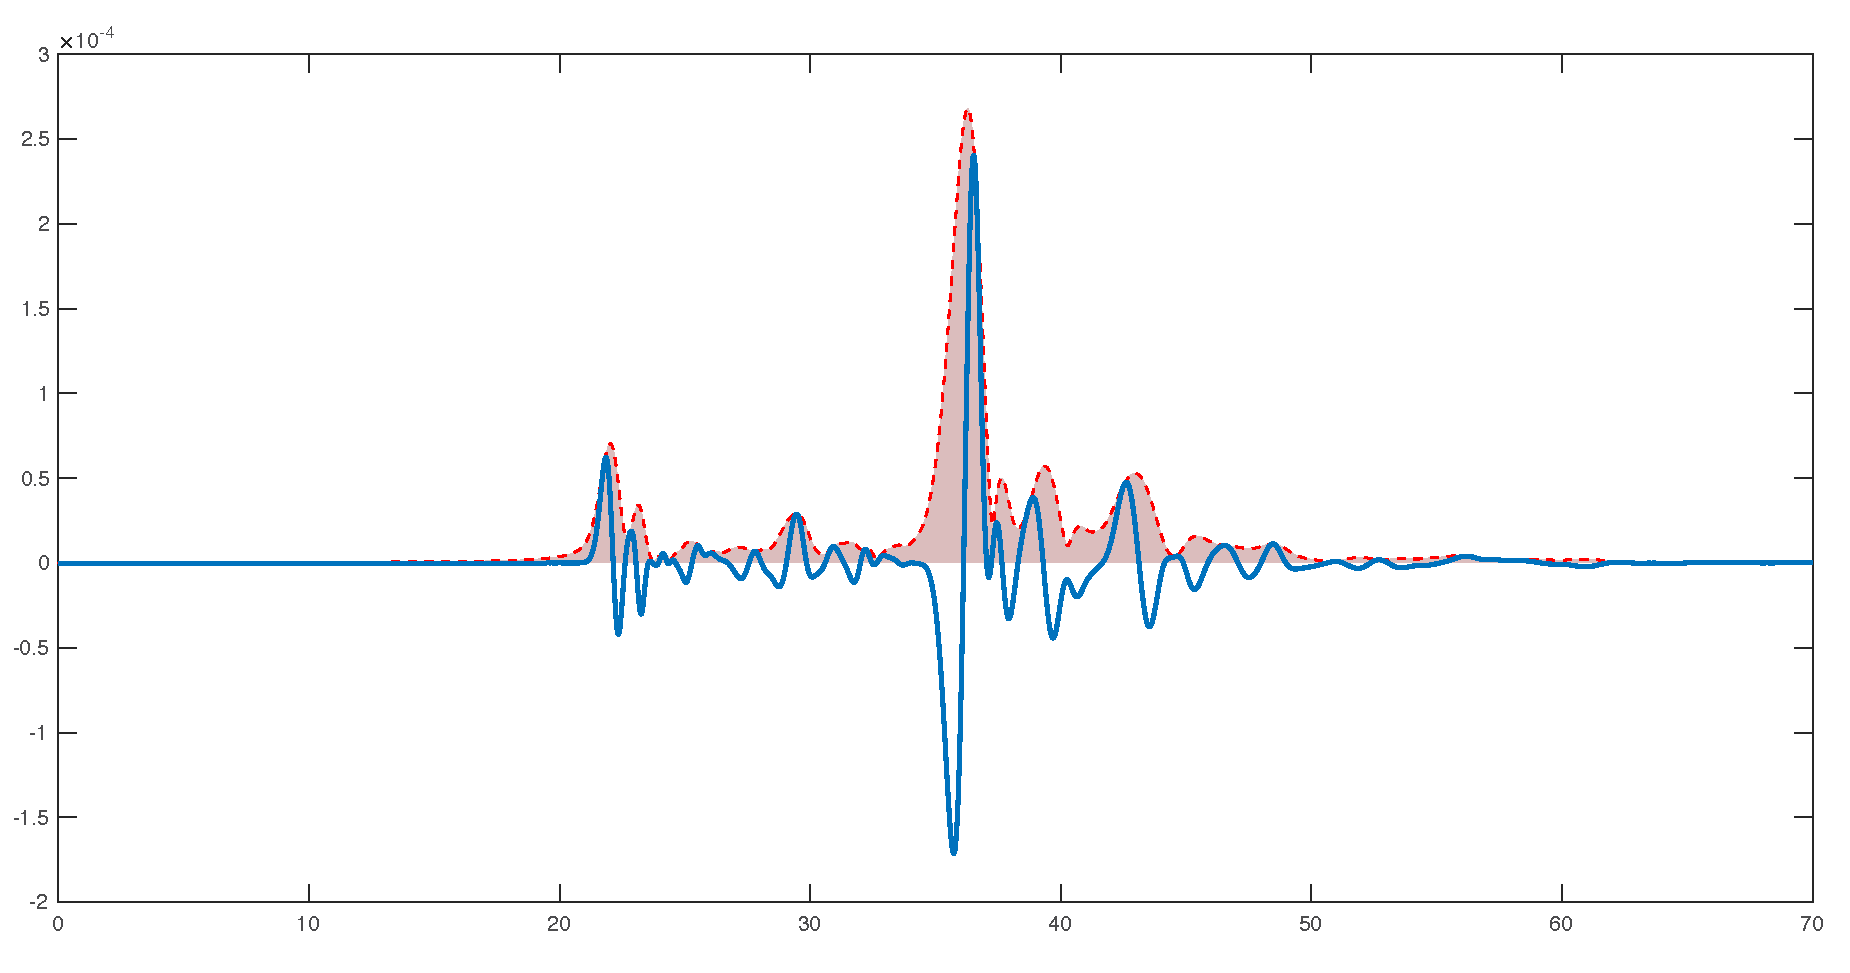
\includegraphics[width=\textwidth]{figures/pdf/signal_envelop.pdf}
    \caption{Example of signal envelop}
    \label{fig:signal_envelop}
\end{figure}




\subsection{Developing sudo-simulators and training process}

We use artificial neural networks to estimate a signal properties (i.e., peak ground acceleration, peak ground velocity, response spectra, and area under signal envelop) of each station based on Q model input parameters (i.e. $c,~\alpha,~and~\beta$). Artificial neural networks (ANNs) are inspired in the human brain. A given network is the combination of different so-called neurons which have certain initial weight and activation functions. One can train a network using available data by means of a process during which the weights and bias values associated with the network's neurons are updated so that these will produce output results with increasingly lower residuals in comparison with the input observations.  Training of an ANN provides the means to avoid repeated demanding computations. ANNs are extensively used in pattern recognition, classification and function regression and other aspects of science \citep[][.] {Hinton2012deep,Baughman2014neural,Graves2013speech,Dahl2012context,Toshev2014deeppose}
ANNs also used in  ground motion prediction \citep{Hong2012observations,Ghaffarzadeh2013neural,paolucci2018broad}. Although some of these previous efforts have shown good and promising results, the alternative conventional simulation methods remained as a better computational alternative. In other words, training of the network was more expensive than running the simulations. This may, however, not be the case for 3D physics-based simulations where one wants to conduct an optimization processes that needs to run the simulation thousands of time.\\
Studying neural network structure and different networks and algorithm are beyond the scope of this study.  In this study we use as simple structure of neural network with 3 input values and 1-8 output values with three hidden layers. We use Feed-Forward Neural Network and Levenberg-Marquardt optimization as a network training function in order to update weight and bias values. We use linear transfer function for the last layers and hyperbolic tangent-sigmoid transfer function for the rest of them. The package is implemented in Matlab programming tool. More network details will be provided in results section. The algorithm divides the data into three sets including: training, validation, and test dataset. Validation dataset is used to stop training process to avoid overfitting during the training process. The test dataset is used after fully training data to analyze the functionality of network. Neural networks' training process, depending on the size of network, are involved with hundreds of thousands of matrix multiplication. Therefore, normalized input values ensure the stability of the network and increase its functionality. We linearly scale the data into $[-1,1]$ using

\begin{equation}
X_{norm} = \frac{2*(X-X_{min})}{(X_{max}-X_{min})}-1
\end{equation}

In general, with increasing training data, the network functionality increases for unseen data and becomes more generalizable. However, in many cases, developing training data can cost considerable amount of computational and/or financial resources. In this study we generate enough training data and study the effect of training data size in network performance. In oder to increase the network accuracy and reduce overfitting we use ensembling method through bagging approach. Going through these process the prediction model predicts the peak values with very high accuracy. 


\subsection{Optimization process}

Having the boundaries of parameters and a cost function, we need to set up an optimization process to search for the best set of parameters to efficiently minimize the cost function. Our preliminary studies (include 2016 scec poster) show that there are not a unique solution for the process and many combination of parameters can be a good candidate. It is understandable because for each station there is a dominant shear wave velocity  in the ray path. Therefore, different combination of parameters where they generate common values for a range of Vs can be acceptable results. Therefore, our cost function can have infinite number of local minimum with acceptable accuracy. In result we need to have a global optimization process to be able to have a good searching strategy in different part of the domain.  Therefore, we use Genetic algorithm as a derivative free single objective method in optimization process. We generate a series of optimal results for each station. These results provide a good understanding of the dominant/effective shear wave velocity for that specific station. \\

\citet{Holland_1973} introduced genetic algorithms (GA). It is not a mathematically guided solution to the problem; rather, It is merely a stochastic, discrete, nonlinear, and highly dimensional search algorithm.We developed a simple GA according \citet{man1996genetic}. Each population includes the quality factors parameters. After evaluating the first set of populations that are basically random parameters in the defined range, the algorithm iteratively defines new populations. Every time that new population is generated it goes through the evaluation process. In the evaluation process which we call it cost or objective function (according to GA nomenclature), it gets the parameters as an input and compute the differences between observation and synthetic. Then it sorts the population according to the best cost (in ascending order). In order to facilitate the GA evolution cycle, two fundamental operators: Crossover and Mutation are required. We use uniform crossover approach as crossover operations. This generates offspring from the parents based on randomly generated crossover mask. 
In this process for each iteration, and for each population, parents exchange the sections to generate the offspring.  At each iteration also in the mutations process, the algorithm randomly picks new value in the defined range. Crossover tends to conserve the genetic information present in the strings. Mutation however is not a conservative operator but capable of generating new building blocks radically. Upon generating new population the algorithm calculate the costs and sorts the population according to score and crossover the best solution with part of other good solutions. Since the best chromosome of the population may fail to reproduce better offspring in the next generation, it is usually combined with elitist strategy such that one or number of the best chromosome can be copied in to the succeeded generation.  Next generation (offspring) is combination of best solutions of previous generation, mutated generation and crossover generation. The cycle of evolution is repeated until a desired termination criterion is reached. In this study we use adaptive feasible and crossover scattered functions as mutation and crossover functions (for more details see \citet{Matlab_optim}).  We defined three termination criteria. Maximum number of iteration, in this case the optimization process regardless of the wellness of the results is terminated,  Fitness limit, in this case the value of fitness function for the best point in the current population is less than or equal to fitness limit; and achieving best score and successive iterations with no produce of better results. 

%In this study the we use the default mutation function (Adaptive Feasible) when there are constraints, randomly generates directions that are adaptive with respect to the last successful or unsuccessful generation. The mutation chooses a direction and step length that satisfies bounds and linear constraints.
%Crossover function (CrossoverFcn) specifies the function that performs the crossover. Do not use with integer problems. You can choose from the following functions:
%Scattered (@crossoverscattered), the default crossover function for problems without linear constraints, creates a random binary vector and selects the genes where the vector is a 1 from the first parent, and the genes where the vector is a 0 from the second parent, and combines the genes to form the child.

%        PopulationType: 'doubleVector'
%             PopInitRange: [2�3 double]
%           PopulationSize: 40
%               EliteCount: 2
%        CrossoverFraction: 0.8000
%           ParetoFraction: []
%       MigrationDirection: 'forward'
%        MigrationInterval: 20
%        MigrationFraction: 0.2000
%              Generations: 20
%                TimeLimit: 600
%             FitnessLimit: 1.0000e-04
%            StallGenLimit: 50
%                StallTest: 'averageChange'
%           StallTimeLimit: 300
%                   TolFun: 1.0000e-06
%                   TolCon: 1.0000e-03
%        InitialPopulation: [1 0.8995 -1]
%            InitialScores: [0�1 double]
%       NonlinConAlgorithm: 'auglag'
%           InitialPenalty: 10
%            PenaltyFactor: 100
%             PlotInterval: 1
%              CreationFcn: @gacreationuniform
%        FitnessScalingFcn: @fitscalingrank
%             SelectionFcn: @selectionstochunif
%             CrossoverFcn: @crossoverscattered
%              MutationFcn: @mutationadaptfeasible
%                  Display: 'final'
%               Vectorized: 'off'
%              UseParallel: 1
%     UserSpecPopInitRange: 0
%           MultiObjective: 0
%                Verbosity: 1


%%%%\input{time_frequency}


In summary we generate a series of training data for the specified earthquake based on different Q-factor parameters. For each station we train a set of neural networks. In an optimization process, we compute a set of parameters that provide the best match with observation. Then we peak the mean value of the observation Q equation and find the closes value to it from training data. We exclude that value from training data and use it as a target value in optimization process. According to the results we pick those velocity ranges that the synthetic optimization test could find the accurate results for them and also the points are in the one standard deviation of the results. Fig.~\ref{fig:Figure_1} represents the processing steps. 

 \begin{figure}
    \centering
    \includegraphics[width=\textwidth]{figures/pdf/Figure_1.pdf}
    \caption{Processing steps}
    \label{fig:Figure_1}
\end{figure}














\section{ Models setup}

In this section, we explain the details of models which are used in this study.  These models include physics-based ground motion simulation domains, seismic sources, \qsvs{} relationships, ANNs as surrogates, and GA optimization process.  

\subsection{Idealized Domains}

To test the proposed method, we use four different idealized domains. Idealized domains are essential because we have a control on shear wave velocity of the domains. This study's idealized domains are homogeneous and layered. Fig.~\ref{fig:3d_domain_scenarios} represents these domains and seismic velocity,density and depth of layers.  The simulation domain is a cubical box (32.8*32.8*8.2~km). All idealized domains have the same source and 17 stations locations. However, they have different velocity models. The homogenous half space (H1) is the simplest one. We add a shallow (256~m) low velocity layer to H1 domain. This Layer adds some complexity to the homogenous domain. We call this domain L1. In order to study the effect of layer thickness in the results, we modify L1 into L2 domain by increasing the depth of low velocity zone from 256 to 1024~m. The last layered domain includes three layers with 2000, 1000, and 500~m/s shear wave velocity, respectively.  

 \begin{figure}[ht]
    \centering
    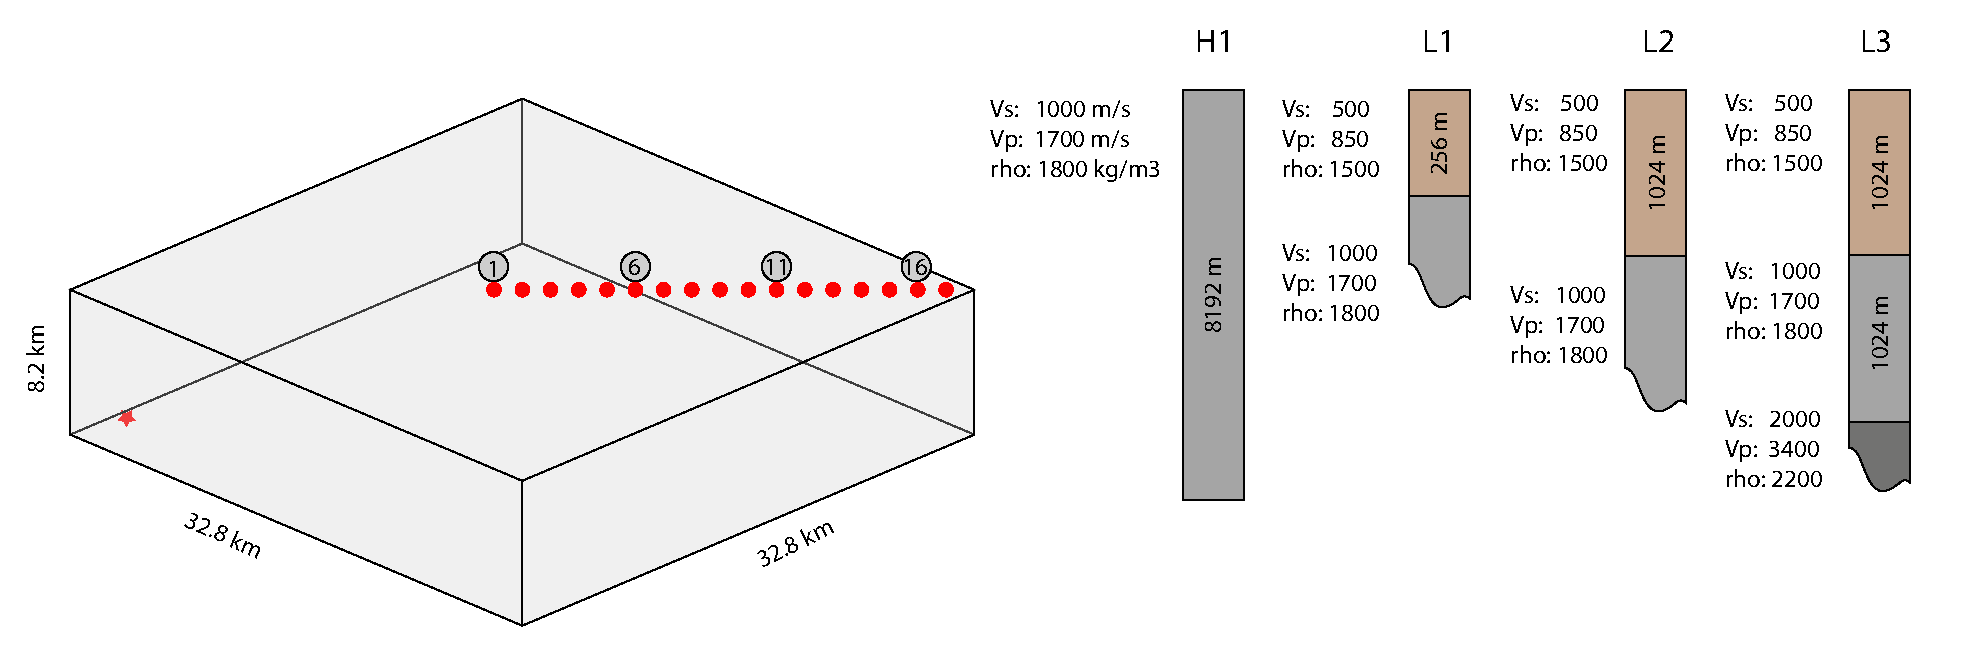
\includegraphics[width=\textwidth]{figures/pdf/Figure_05.pdf}
    \caption{Idealized domains to test the proposed method. Earthquake source is shown with star (2048,2048,7168). Station are at the surface and the numbers are referred in the text. All four idealized case share the same domain dimension with different velocity models.}
    \label{fig:3d_domain_scenarios}
\end{figure}

We run ground motion simulations for each of these domains based on known damping parameters. Using the synthetic generated data as a target values at each station we search for the initially used \qsvs{} relationship parameters to see if the optimization process can find the initially used parameters. The idealized domains are used to confirm the accuracy of the optimization process. We modeled each seismic event with a point source model with seismic moment that is tailored for magnitude $Mw~3.5$. Fig.~\ref{fig:record_section_1000} represents the record section of NS horizontal component for peak ground velocity in H1 domain. The record of each stations are shown according to their hypocenteral distance from the source. Dashed lines show \vp{} and \vs{} arrival times. Peak amplitude of P and S wave of each station can be detected after dashed lines. 

  \begin{figure}[ht]
    \centering
    \includegraphics[width=0.8\textwidth]{figures/pdf/Figure_06.pdf}
    \caption{Record section of NS component of H1 domain. Amplitudes are scaled for better representations.}
    \label{fig:record_section_1000}
\end{figure}

Fig.\ref{fig:record_section_2000_1000_500} represents the record section of NS horizontal component for peak ground velocity in L3 domain. Dashed lines show \vs{} for 2000 and 1000~m/s. 

  \begin{figure}[ht]
    \centering
    \includegraphics[width=0.8\textwidth]{figures/pdf/Figure_07.pdf}
    \caption{Record section of NS component of L3 domain. Amplitudes are scaled for better representations.}
    \label{fig:record_section_2000_1000_500}
\end{figure}

Reflected waves from different layer makes it difficult to choose the peak ground velocity for S wave arrival. The complexity of the other two idealized domains lay between the shown results. 

\subsection{Heterogenous Domain}

Heterogenous domain has a significant difference from idealized ones. In heterogeneous domains, we do not know the effective shear wave velocity of each station. Each station can have some range of effective shear wave velocity. In a heterogeneous domain, depending on effective shear velocity of each station, waves arrive in different times. The heterogeneous region used in this study has greater Los angeles area and also it includes many small basins in different parts. Numerous earthquake recorded in this area and different ground motion simulation studies are conducted for the region for different events; and several velocity models are developed \citep[e.g., see][]{Taborda_2013_BSSA,Taborda_2014_BSSA,Small_2017_SRL}. Fig.~\ref{fig:Figure_stations} shows the  heterogeneous domain and stations location. 

 \begin{figure}[ht]
    \centering
    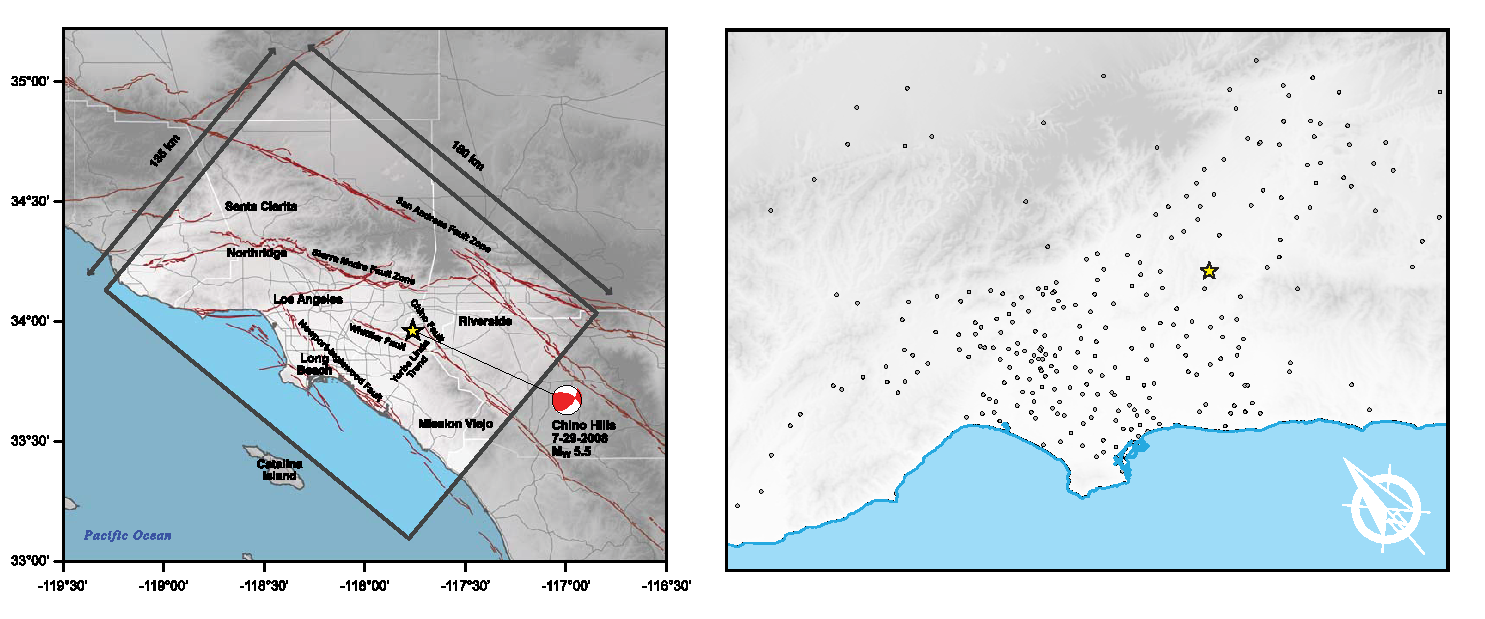
\includegraphics[width=\textwidth]{figures/pdf/Figure_08.pdf}
    \caption{Left: Region of interest and epicentral location of the 2008 Chino Hills earthquake. Major quaternary faults in the area are shown in the back along with the main roads and county divisions. Right: Simulation are of interest. Dots indicate the location of the 262 stations considered in this study for optimization process. {\color{red} Stations that are used in the study will be marked on this figure.}}
    \label{fig:Figure_stations}
\end{figure}

In order to test the methodology with real observational data, we use 2008 $Mw~5.4$  ChinoHills earthquake as an observation platform. Chino Hills earthquake is recorded at more than 300 stations. however we only use the Center for Engineering Strong Motion Data, where there are 262 stations within this study simulation box. We modeled the seismic event with a point source model according to \citep{Taborda_2016_GJI}. Table~\ref{tab:event_details}  and Table~\ref{tab:sim_param} represent the event and simulation details, respectively. 


\begin{table}[ht]
\centering
\caption{Event details}
\label{tab:event_details}
\renewcommand{\arraystretch}{0.75}
\begin{tabular}{lr}
\\ \hline
Name                                 &   Chino Hills                          \\
Origin Time                        & 29 July 2008 , 11:42 AM             \\
Magnitude                          &  Mw 5.4            \\
Moment                             & 1.566751e+17 Nm             \\
Location/Depth                  &  -117.7613 33.9530 14.7 $Km$    \\
Strike/Dip/Rake                 & 47/51/32                                   \\
3D Crustal Model              & SCEC CVM-S4.26                   \\
Source Model                   & Point Source                                  \\ \hline
\end{tabular}
\end{table}


\begin{table}[ht]
\centering
\caption{Simulation Parameters}
\label{tab:sim_param}
\renewcommand{\arraystretch}{0.75}
\begin{tabular}{lr}
\\ \hline
Domain                              &                              \\
~~Length/Width/Depth       & 180,135,61.875 km \\
~~Southwest corner          & -119.288842, 34.120549             \\
~~Northwest corner           & -118.354016, 35.061096             \\
~~Northeast corner            & -116.846030, 34.025873              \\
~~Southeast corner           & -117.780976, 33.096503               \\
~~Rotation Angle               & 39.9 \\
~~Studied records             & 262 \\
Spatial Resolution              &    \\
~~Maximum frequency     & 1 $Hz$ \\
~~Minimum $V_s$            & 350 m/s \\
~~Points per wavelength   & $9\leq p < 14$\\
~~Minimum size element   & 21.9727 $m$\\
~~Maximum size element   & 351.5625 $m$\\
~~Number of elements       & 157209765 \\
~~Number of nodes            & 180080443 \\
~~Number of dangling nodes & 23681911 \\
Time resolution  & \\
~~Simulation $\Delta$t & 0.002 \\
~~Simulation time & 100 s\\ \hline
\end{tabular}
\end{table}

\subsection{Artificial Neural Networks}

We use 1000 combination of randomly generated $C$, $\alpha$, and $\beta$ to develop training data for ANNs. Each training data is the result of running a physics-based ground motion simulation on the domains. Fig.~\ref{fig:Figure_training_data_statistics} shows statistical distribution of the generated data.

 \begin{figure}[ht]
    \centering
    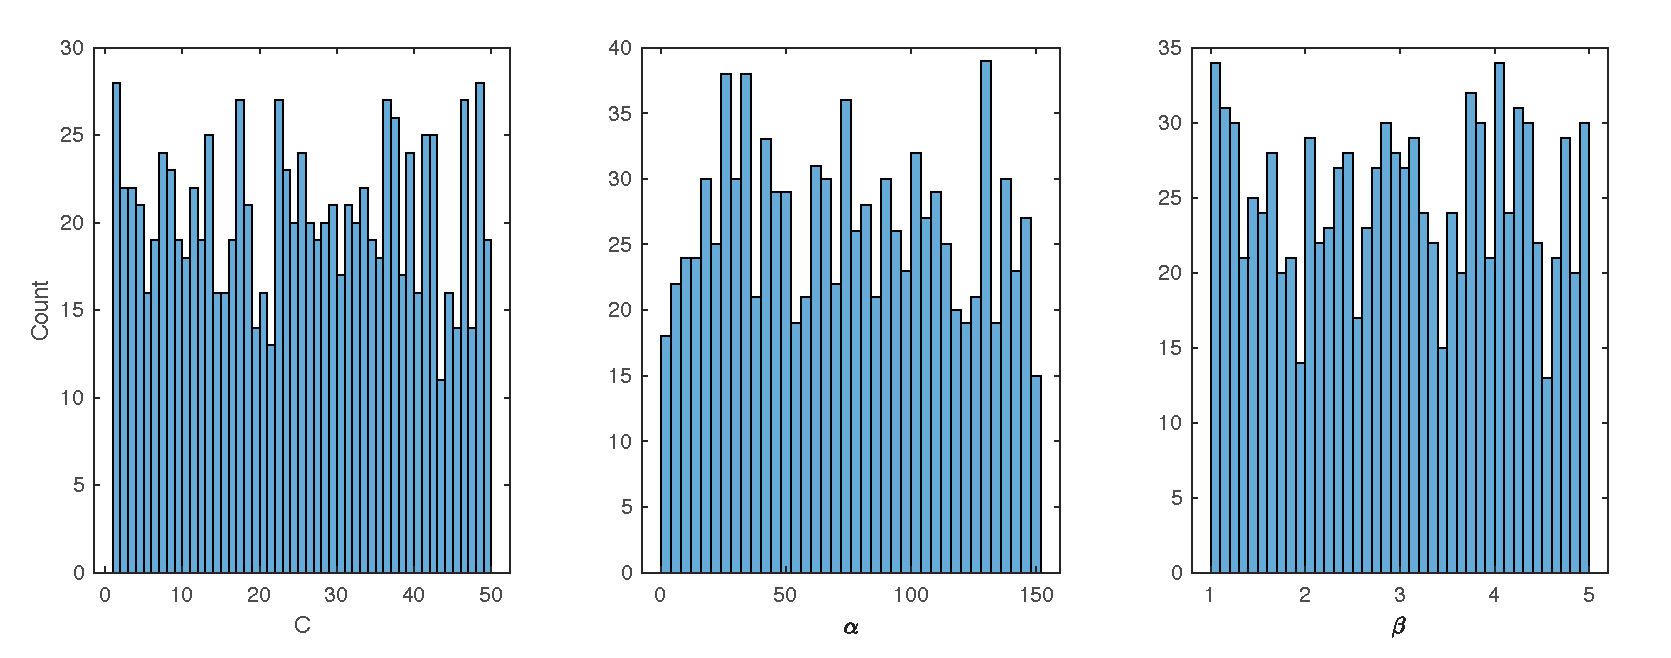
\includegraphics[width=\textwidth]{figures/pdf/Figure_09.pdf}
    \caption{Distribution of \qsvs{} relationship input parameters (i.e. $C$, $\alpha$, and $\beta$) which are used in generating 1000 training data for ANNs.}
    \label{fig:Figure_training_data_statistics}
\end{figure}

 Our analyses show that, defining higher $C$ values (more than 50) compromise the functionality of the network. The reason is, higher $Q$ values provide almost the same signal parameters independent of the input values. Moreover, according to Table~\ref{tab:table_qs} almost all models proposed lower $Q$ values for low velocity zones. Most of previous studies show that $Q$ value increases with increasing shear wave velocity, therefore, we consider $\beta$ to be in the the range of $[1,5]$. Suggested values for $\alpha$, mostly, is between 50--100; we broaden the search domain and use $[0,150]$ as a range of $\alpha$ variation. Therefore, each station of simulation has 1000 training data. Fig.~\ref{fig:Figure_training_data} illustrates that the generated training data can cover almost the whole range of \qsvs{} relationships. Values of Table~\ref{tab:QsVstable} and Fig.~\ref{fig:Figure_q_models} are shown as a thicker black line. The simulation \vsmin{}=350~m/s, therefore, the part of a line which is partially not covered is out of the target velocity zone of this study. 

 \begin{figure}[ht]
    \centering
    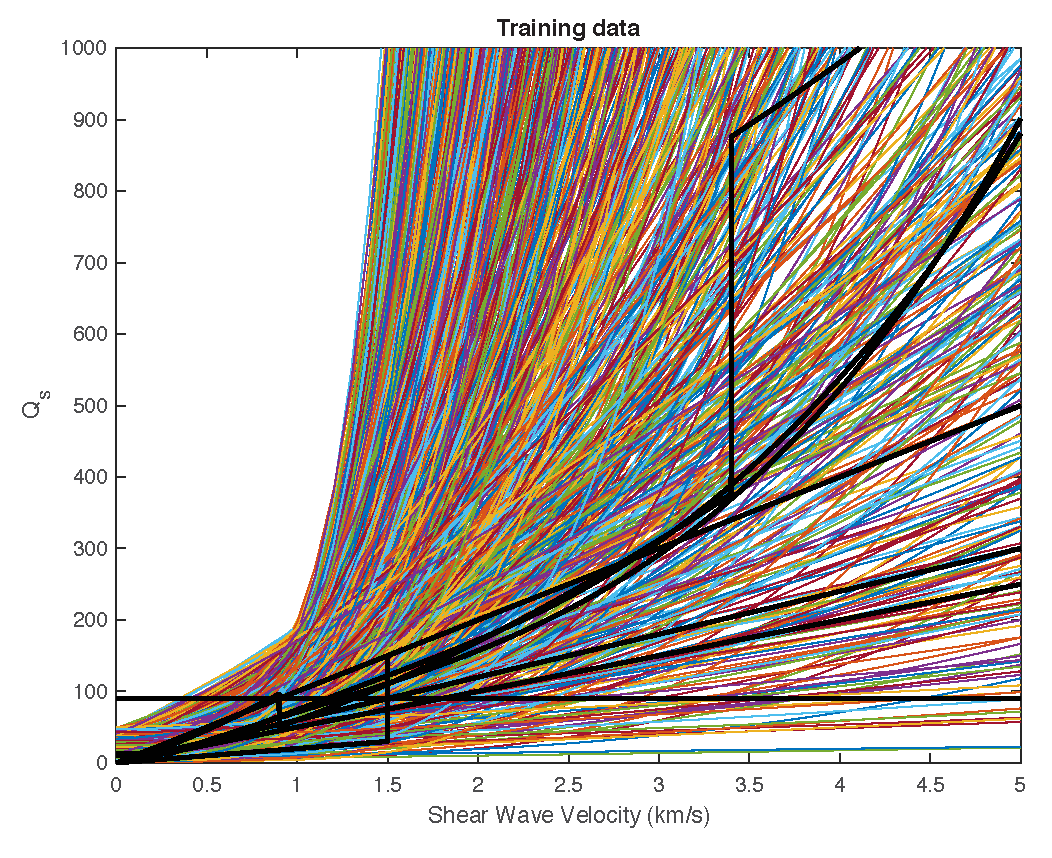
\includegraphics[width=0.5\textwidth]{figures/pdf/Figure_10.pdf}
    \caption{Training data is generated based on 1000 random combination of $C$, $\alpha$, and $\beta$. For statistical distribution of the input parameters refer to Fig.~\ref{fig:Figure_training_data_statistics}. Thick black lines are transferred from Fig.~\ref{fig:Figure_q_models} and represented only for comparison purposes.}
    \label{fig:Figure_training_data}
\end{figure}

 Fig.~\ref{fig:Figure_training_performance} represents the training performance for one of the networks (predicting eight output parameters).


  \begin{figure}[ht]
    \centering
    \includegraphics[width=\textwidth]{figures/pdf/Figure_11.pdf}
    \caption{a) Train, Validation, and Test performance. The circle shows the start of RMSE value for the validation dataset which means overfitting occurs. b) Error histogram}
    \label{fig:Figure_training_performance}
\end{figure}

Fig.~\ref{fig:Figure_training_performance}.a shows the performance of the network for train, validation, and test datasets with respect to epoch.  In the presented training session, after epoch 140, overfitting occurs because training data error decreases, however, validation data error increases. Training session stops based on user defined termination criteria. In this example, since ANN cannot overcome the overfitting problem (validation dataset error still not improving) after 100 more iterations, the learning process stops and the best network that acquired at epoch 140 is returned to the user. Toward bagging approach, we generate 10 different ANNs and use the average value of their predictions. For each ANN, training and validation data are randomly set. Therefore, these networks are trained for different combination of data. Fig.~\ref{fig:Figure_ANN_num_training_data_sens}.a shows that increasing the number of training data, in general, reduce the RMSE for test dataset. Fig.~\ref{fig:Figure_ANN_num_training_data_sens}.b represents accuracy of training network with 100, 400, and 1000 training data on the test dataset. In the figure, the red cross shows results of each individual ANN, the blue circles represent the value of observations and green stars are average of 10 ANNs. In the case with 100 training data, each individual network results (red crosses) is far from the actual value (blue circles), however, bagging approach average them out (green stars) which leads to better fit with actual value. 

  \begin{figure}[ht]
    \centering
    \includegraphics[width=0.8\textwidth]{figures/pdf/Figure_12.pdf}
    \caption{a) Variation of RMSE with increasing number of training data; b)Examples of predicting target value in actual simulation with 100, 400, and 1000 training data. The networks are tested using testing dataset. RMSE scores computed using bagging results.}
    \label{fig:Figure_ANN_num_training_data_sens}
\end{figure}

\subsection{Variation of Alternative Metric Results}
As we mentioned earlier, defining alternative metrics increase signal uniqueness. The variation of input parameters (i.e., $C$,$\alpha$,and $\beta$) are constant for all signal metrics. Since we have all training data and respective ground motion results for each domain, we take a look at variation of alternative metrics for each metric and domain. We use coefficient of variation (CV) as a measure of relative variability of metrics. Since input parameters are the same for all signals and simulation we can safely compare CV for different metrics without further analysis. Coefficient of variation is defined as 

\begin{equation}
CV=\sigma/\mu * 100. 
\end{equation}

High CV indicates that the metric is very sensible to input parameters and provides high variability around the mean value. As a result, high CV means better training of ANN and consequently efficient optimization process. Fig.~\ref{fig:metrics_sensitivity} shows CV for 4 different stations of idealized domains. 

  \begin{figure}[ht]
    \centering
    \includegraphics[width=0.8\textwidth]{figures/pdf/Figure_13.pdf}
    \caption{Coefficient of Variation of different metrics for 1000 training data. Symbols indicates different stations. See Fig.~\ref{fig:3d_domain_scenarios} for stations location.}
    \label{fig:metrics_sensitivity}
\end{figure}


Several points are worth mentioning from Fig.~\ref{fig:metrics_sensitivity}. In all domains, CV increases with increasing distance from source. It suggests the idea that far stations can be trained more accurately and they are much more sensitive to the variation of input parameters. The results prove to be true. As distance of stations increases from source, waves have more time to travel in the medium and this means more time to get affected through domain anelasitisiy. In the simple cases (H1,L1, and L2) response spectra at 1 second (SA1) is more variable, whereas in complicated case (L3) the envelop becomes important. 




%Testing of the proposed method is inspired from checkerboard resolution tests idea from inversion studies \citep[e.g., see][]{liang2008ambient}. 




\section{Results}
In this section we test the proposed method on the models. The first idealized domain is a homogenous domain with shear wave velocity of $1000 km/s$. For more information about domain details and stations location see Fig.\ref{fig:3d_domain_scenarios}. Simulation record section shows a very clean arrivals (see Fig.\ref{fig:record_section_1000}.) We train the networks with 1000 set of input parameters. In this case we use PGV of north--south component in optimization process( results for other horizontal components or a combination of them are similar.)  We also generate a set of input parameters as a synthetic observation. The optimization algorithm search for parameters that are the best fit with synthetic observation.  Fig.~\ref{fig:station_1_1000_H1} shows the results of optimization process. For each station we repeat the optimization 50 times. We expect to see at each station, for the effective shear wave velocity (here \vs{}=1000~m/s), the optimized parameters and the target parameters $Q$ are very close to each other if not the same. 

  \begin{figure}[ht]
    \centering
    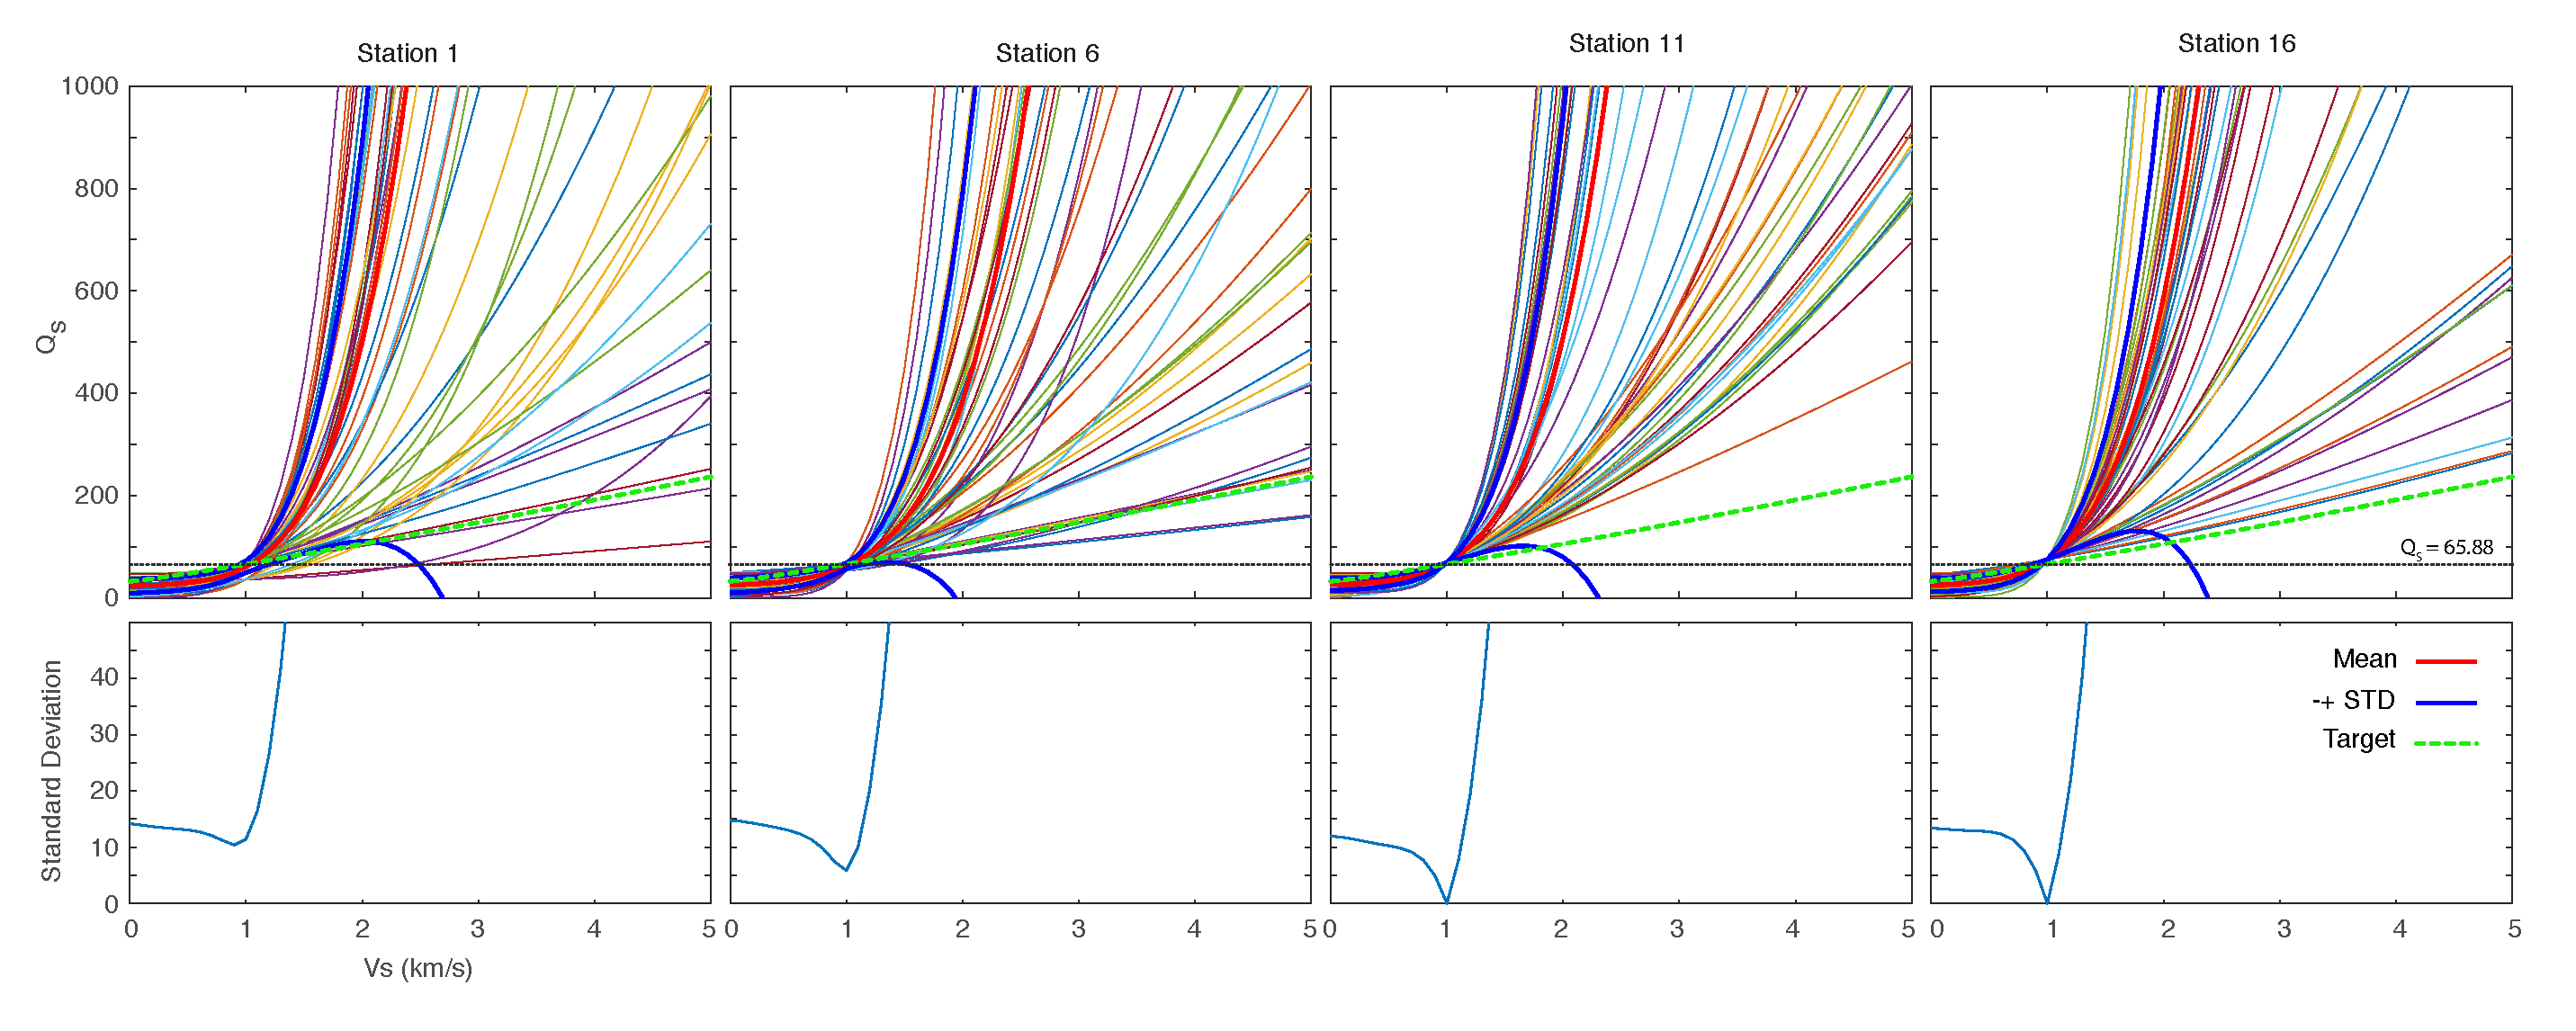
\includegraphics[width=\textwidth]{figures/pdf/Figure_14-H1-pgv.pdf}
    \caption{Results of 50 optimized solutions for homogeneous (H1) domain for 4 stations. The target simulation results are generated based on \qs{}$=32.17+33.71V_{S}^{1.12}$. In this simulation domain (\vs{}=1000~m/s), \qs{}=65.88}
    \label{fig:station_1_1000_H1}
\end{figure}

This figure shows stations 1,6,11, and 16. Standard deviation values which are shown at the bottom of the each stations are indications of convergence of the solutions. We expect to see a very small standard deviation at \vs{}=1000~m/s. Values of standard deviation is decreased at that \vs{}, however,  only station 11 and 16 have a very converged solutions. That is understandable, because at the closer stations the wave does not have chance to travel enough to capture the anelastic damping characteristics. The parameters that are used to generate the target values are shown with green thick dashed line. The convergence points are coincides with target value parameters at \vs{}=1000~m/s or is very close to it. This test gives the idea that for simple case if we can accurately pick the peak ground velocity, at considerable distance from the source, our optimization process can accurately estimate the $Q$ value for effective shear wave velocity by converging at that point. Also it can locate the $Q$ value with acceptable accuracy.
We add a shallow low velocity zone to the H1 domain. Fig.~\ref{fig:station_1_1000_500_L1} shows the results of optimization process. According to the results, as we observed in the homogeneous domain, the closes station to the source is not well converged, with increasing distance standard deviation decreases and also in mid-distance we can see effective shear wave velocity is in the range of 900--1000~m/s whereas at far stations with respect to the source the effective shear wave velocity is 1000~m/s. Obviously for far stations the wave are propagated more in the high velocity zone and are highly affected from that.   

  \begin{figure}[ht]
    \centering
    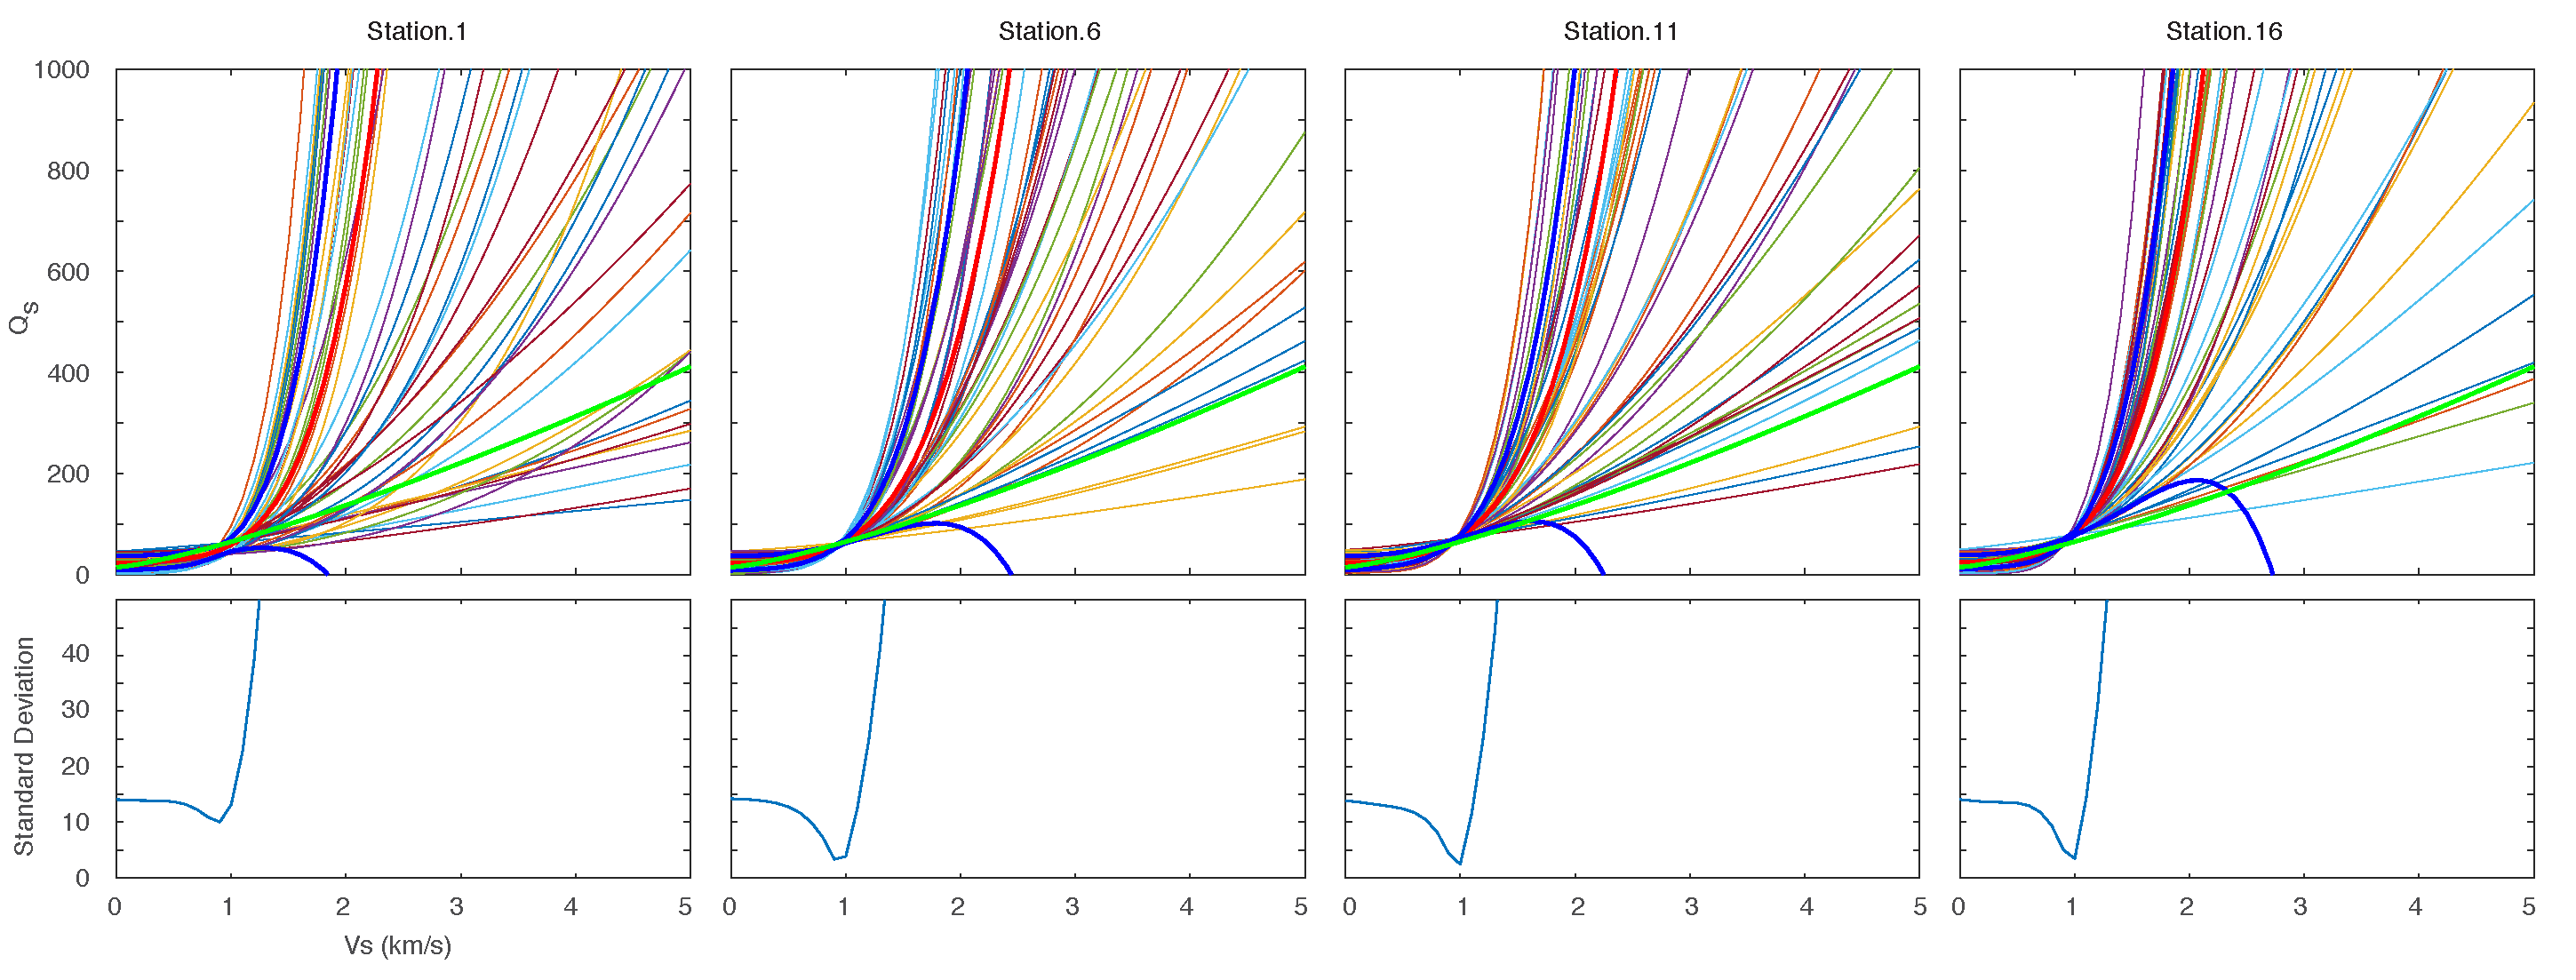
\includegraphics[width=\textwidth]{figures/pdf/Figure_15-L1-pgv.pdf}
    \caption{Results of 50 optimized solutions for Layered (L1) domain for 4 stations.  The target simulation results are generated based on \qs{}$=14.44+50.61V_{S}^{1.28}$. $Q_{S1000}$==65.05 is shown as a reference for \vs{}=1000~m/s}
    \label{fig:station_1_1000_500_L1}
\end{figure}

It is worth mentioning that effective shear wave velocity that is detected in this idealized scenario is not used in the simulation domain. However, the $Q$ value that is detected for that velocity coincides with the initial \qsvs{} relationship that is used.  The dashed green line is the parameters that we have used for developing synthetic observation values. Ideally, all stations, at their convergence point, should coincides with the line. Station 1 has a very weak convergence rate. Station 6, on the other hand, has a acceptable convergence in solution and also detect the initial parameters (dashed line). Station 11 and 16 have very sharp convergence, but the convergence point has a small difference with initial parameters $Q$ values. According to this results, we can say for this velocity and source model if we use PGV of north--south component as a determining metric, Station 6 most probably will detect the $Q$ parameters.
We increase the depth of low velocity zone of L1 domain (from 256 to 1024 m) to see if the effective shear wave velocities of each stations have considerable changes. Fig.~\ref{fig:station_1_1000_500_2_L2} shows the results of optimization process. The results show that the effective shear wave velocity becomes a little less than $1000~m/s$. It is understandable; because in this scenario the $500~m/s$ low velocity zone can have more effects on propagated waves. In this domain, Station 6 and 11 have good convergence and also could accurately detect the initial $Q$ parameters. 

  \begin{figure}[ht]
    \centering
    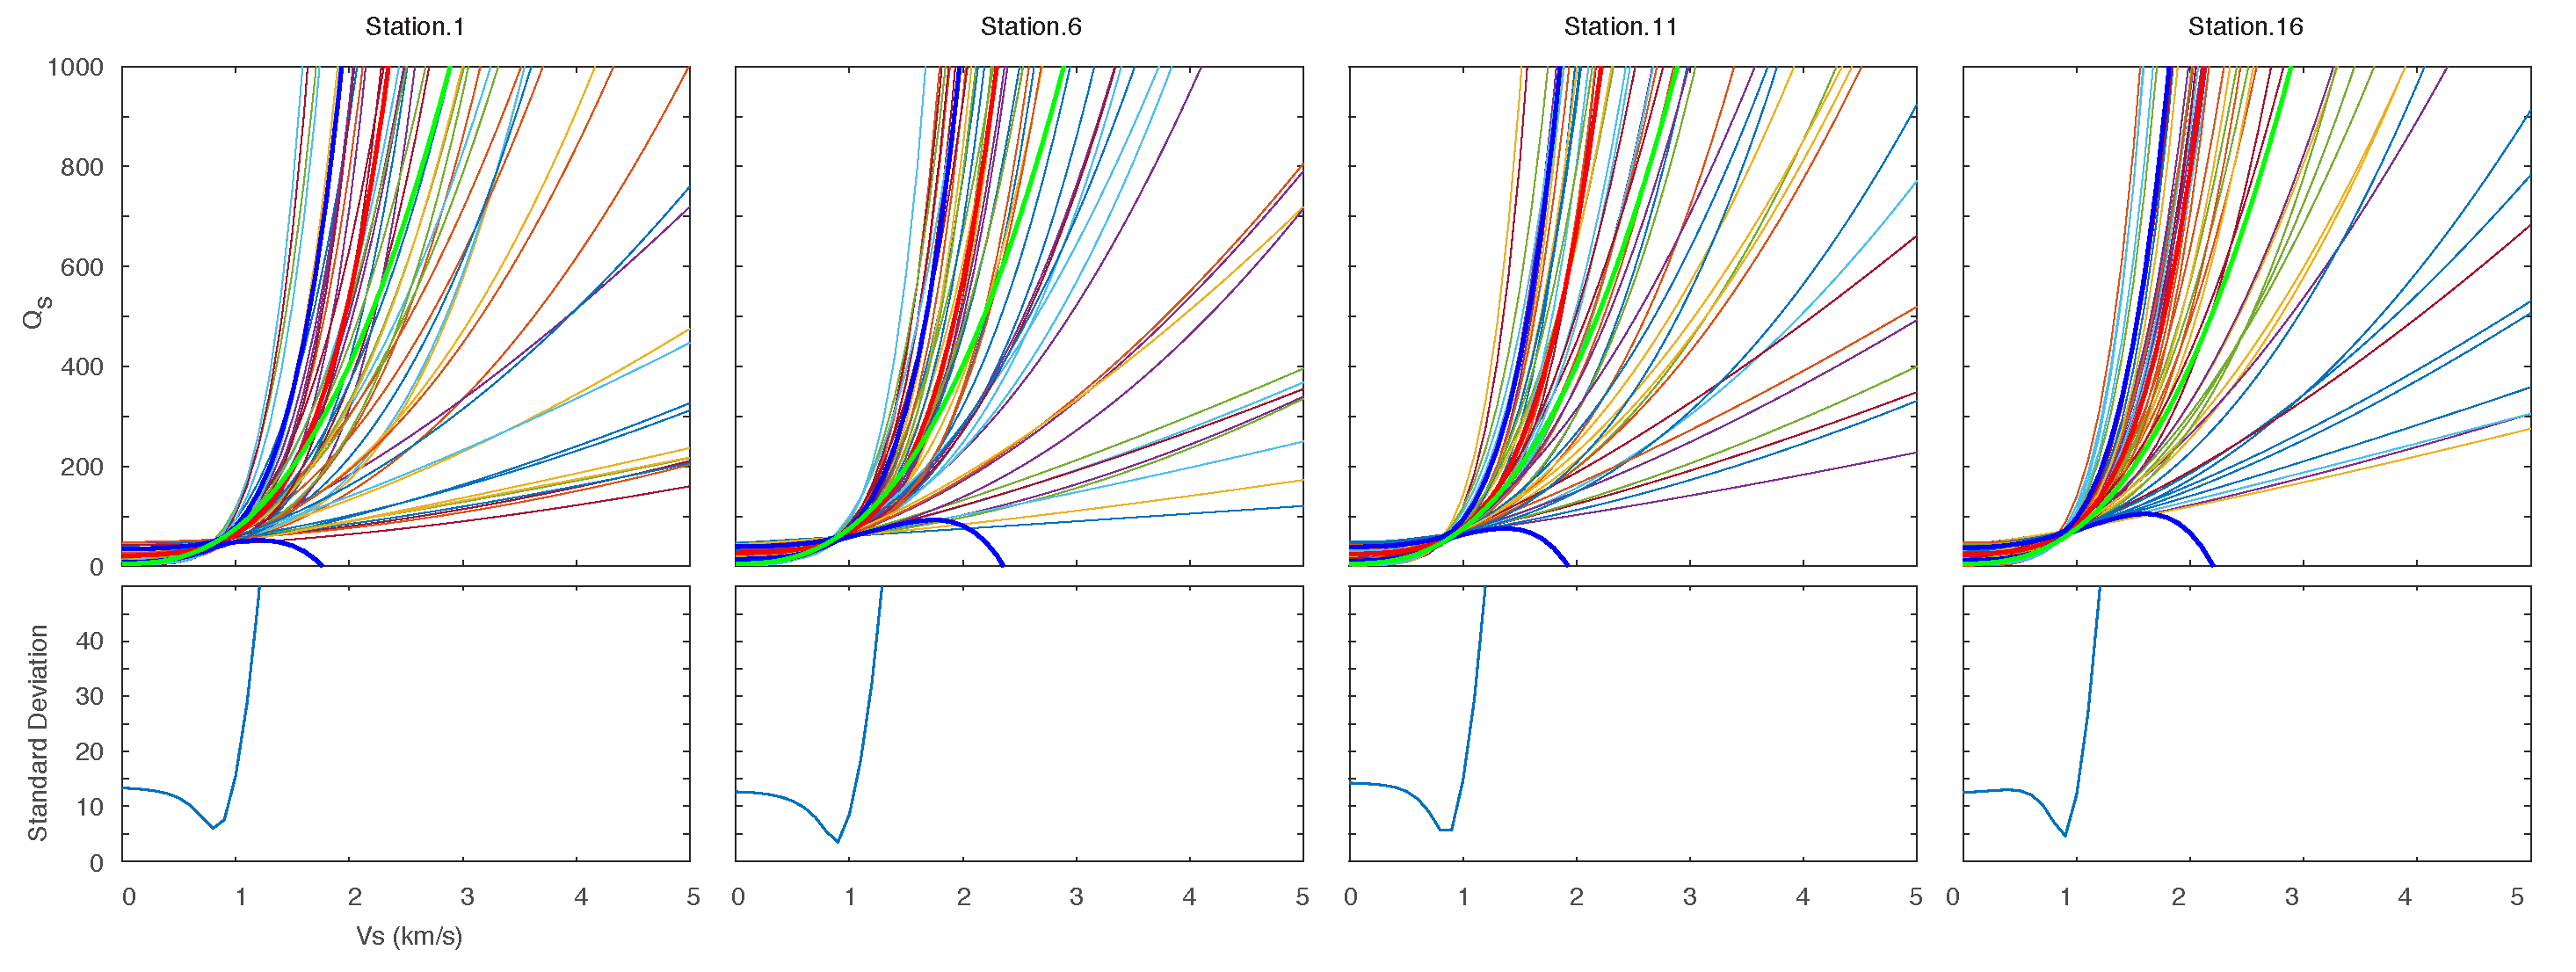
\includegraphics[width=\textwidth]{figures/pdf/Figure_16-L2-pgv.pdf}
    \caption{Results of 50 optimized solutions for Layered (L2) domain for 4 stations. The target simulation results are generated based on \qs{}$=5.21+70.11V_{S}^{2.50}$. $Q_{S1000}=$75.32 is shown as a reference for \vs{}$=$1000~m/s}
    \label{fig:station_1_1000_500_2_L2}
\end{figure}
 

We tried another idealized layered profile with three different layers. According to Fig.~\ref{fig:station_1_2000_1000_500_L3_nt}, with increasing distance from source (Station 1 to 16 ), effective shear wave velocity (i.e., minimum value of standard deviation) is shifting from lower velocity to higher velocity ( m/s to m/s). Far stations records are more affected with high velocity zone. 
 
  \begin{figure}[ht]
    \centering
    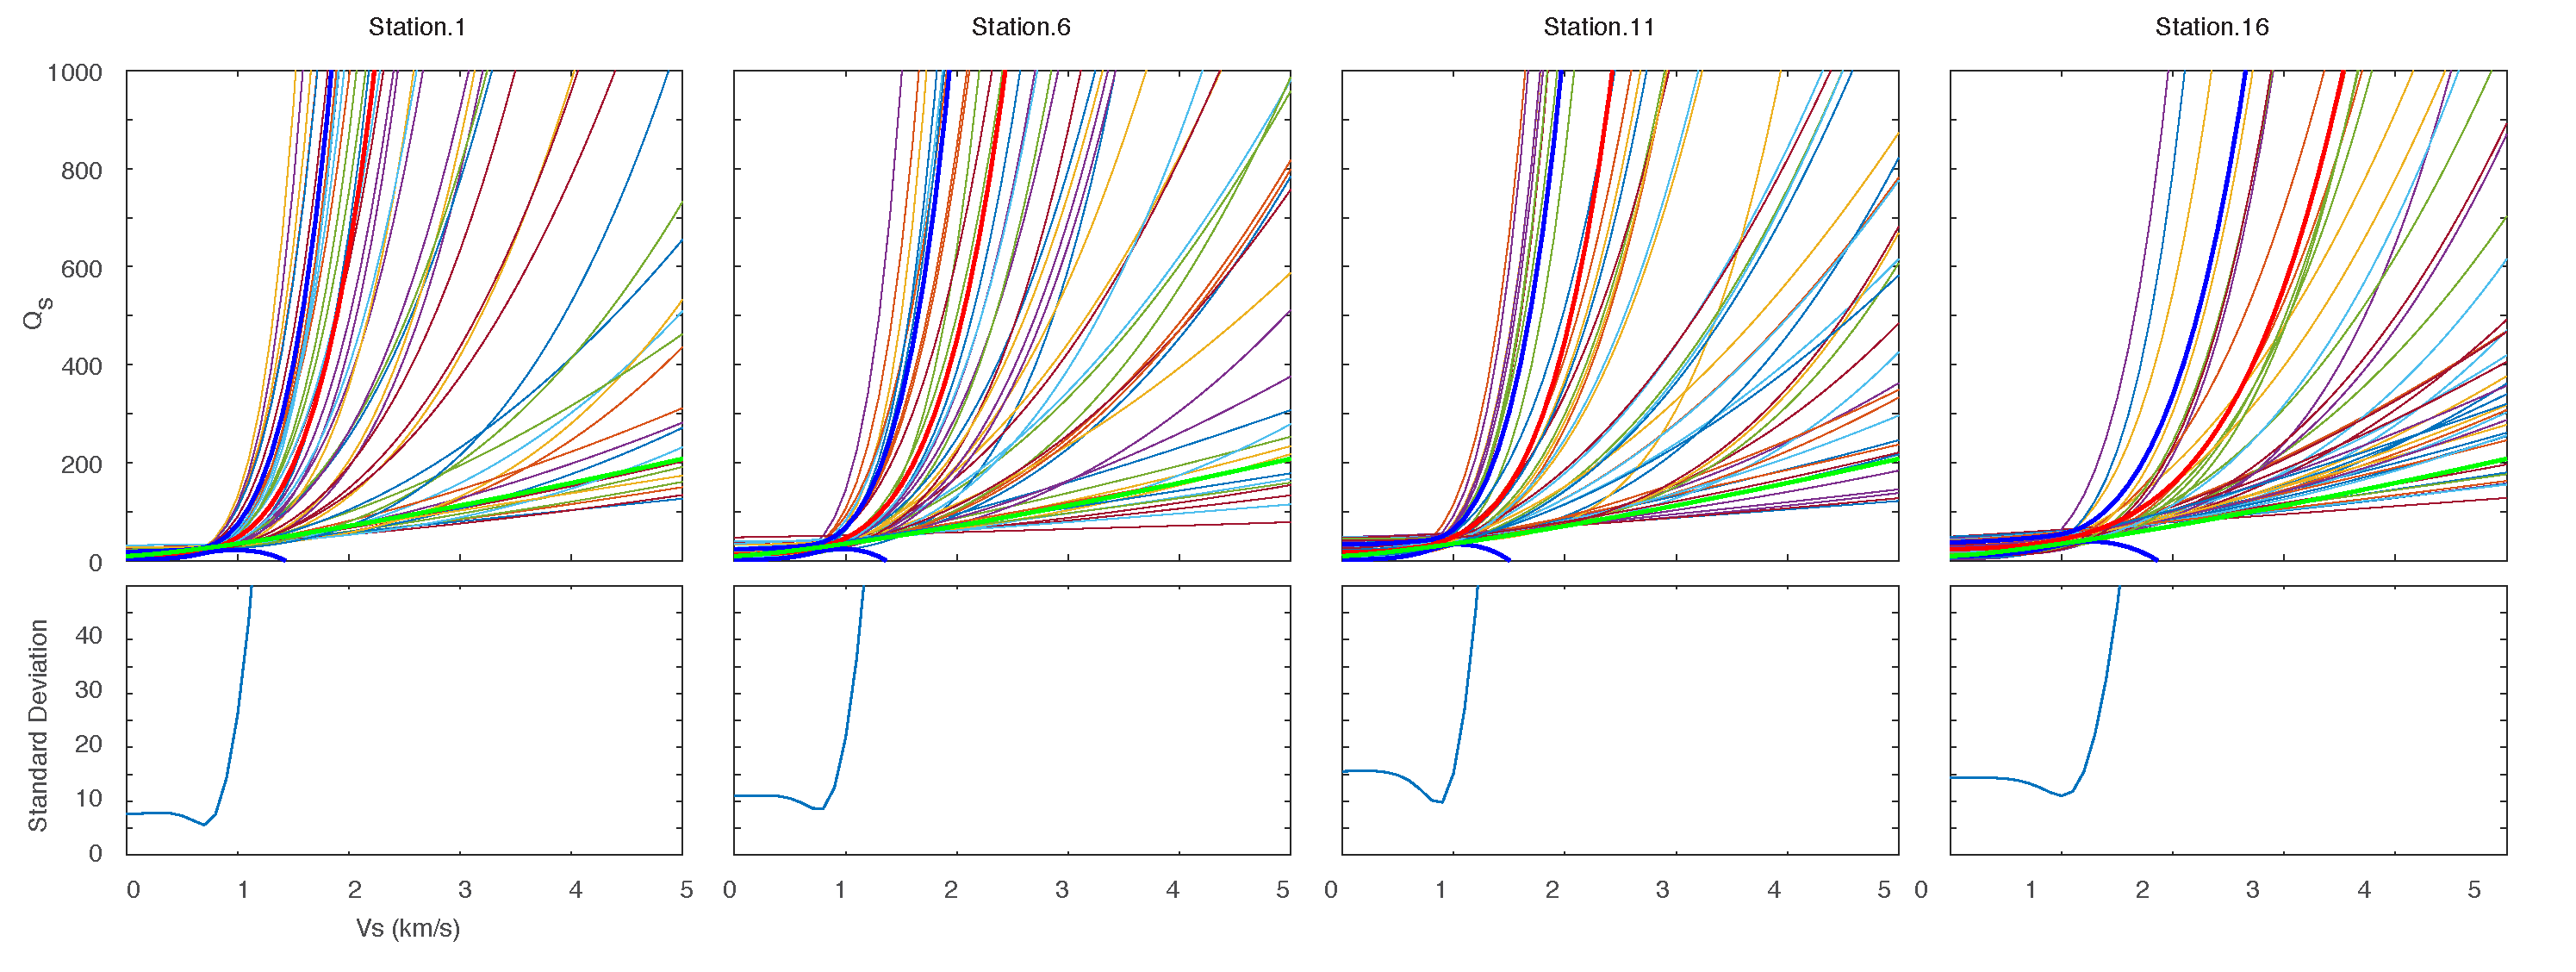
\includegraphics[width=\textwidth]{figures/pdf/Figure_17-L3-pgv.pdf}
    \caption{Results of 50 optimized solutions for Layered (L3) domain for 4 stations. The target simulation results are generated based on \qs{}$=9.28+25.31V_{S}^{1.28}$. $Q_{S1000}=$34.59 and $Q_{S2000}=$70.74 are shown as a reference for \vs{}=1000 and 2000~m/s, respectively}
    \label{fig:station_1_2000_1000_500_L3_nt}
\end{figure}

However, in this test, we do not see a good convergence rate. The standard deviation of the optimum results around the dominant shear wave velocity is slightly lower, but it is not as sharp as the simpler domains (e.g., H1). We achieved similar results for heterogeneous domain, as well. With increasing domain complexities, determination of effective shear wave velocity is not as sharp as before. It suggests that peak ground velocity may not be enough to estimate the results. Please note that the idealized scenarios do not have noise. Complex geological features (velocity models) make PGV less sensitive to input values. Therefore, we use the second ANN structure where it estimates PGV, PGA, SA1, and Venv for two horizontal components. Fig.~\ref{fig:station_8_param_2000_1000_500} shows the optimization results with using 8 metrics. 

  \begin{figure}[ht]
    \centering
    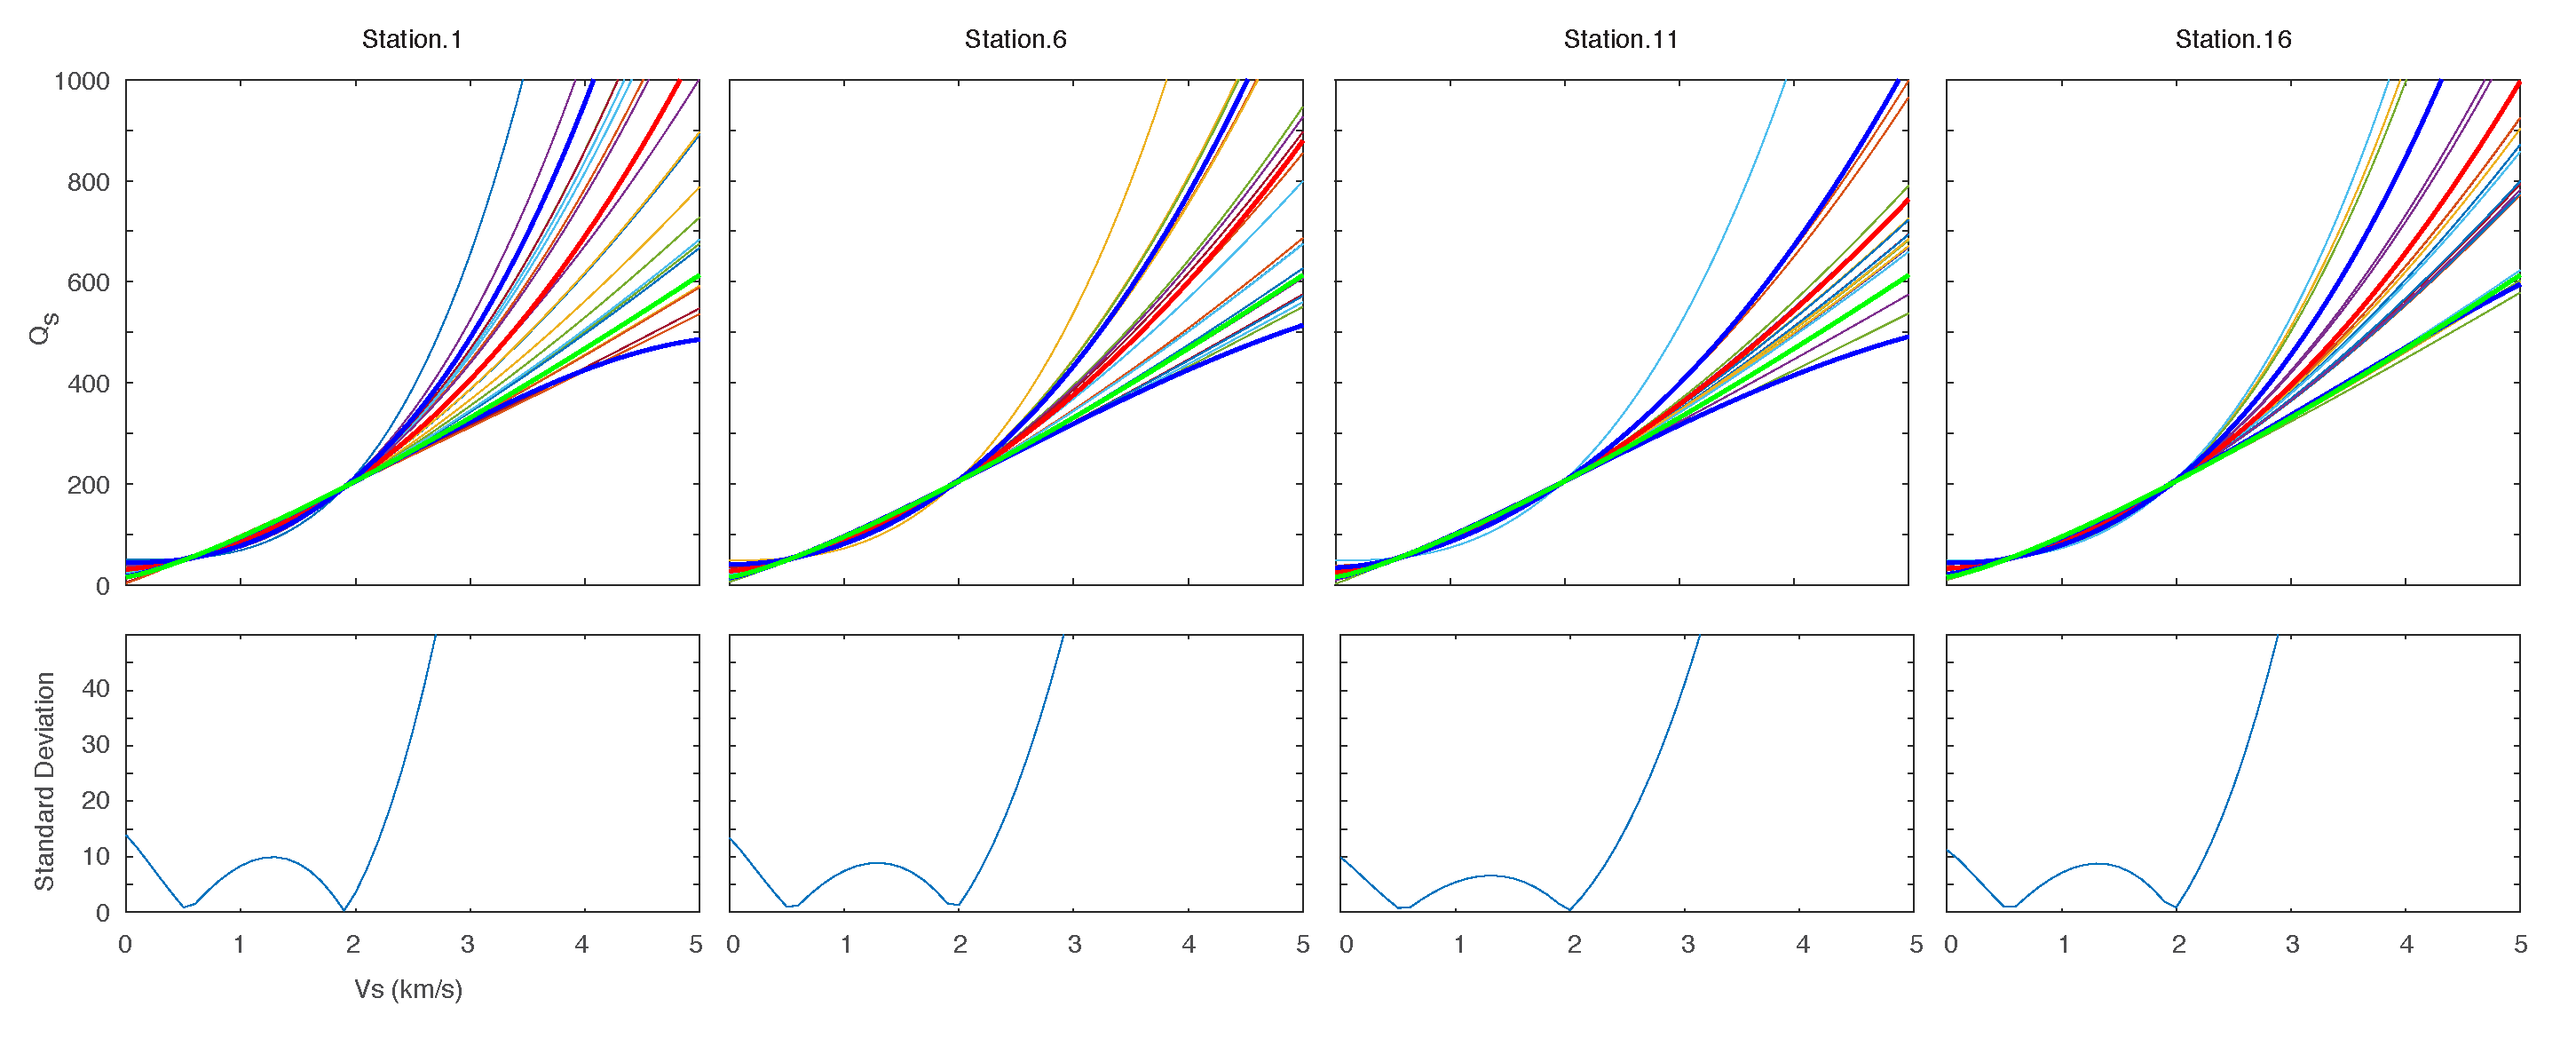
\includegraphics[width=\textwidth]{figures/pdf/Figure_18-L3-8metric.pdf}
    \caption{SA1, PGV, PGA, Env for NS and EW component. Domain(L3). The target simulation results are generated based on \qs{}=$15.12+80.00V_{S}^{1.25}$. $Q_{S500}=$48.76, $Q_{S1000}=$95.12, and $Q_{S2000}$=205.40 are shown as a reference for \vs{}=500, 1000, and 2000~m/s, respectively.}
    \label{fig:station_8_param_2000_1000_500}
\end{figure}

There is a significant improvement in the results. The algorithm can locate two ranges of effective shear wave velocities which are 500 and 2000~m/s in all stations. The results are not accurate for 1000~m/s. In this case, the current metrics and problem setup cannot retrieve valuable information for \vs{}=1000~m/s. This does not compromise the proposed method. The positive factor about the proposed method is that we know before hand that we cannot be confident about the results of \vs{}=1000~m/s. However, the results for \vs{}=500 and 2000~m/s are accurate. 
In idealized domains we show that the proposed method can locate a range of effective shear wave velocity and also accurately estimate the $Q$ values. Since idealized domains have up to three different soil layers. At the most elaborate case we will have three $Q$ values with respect to three effective shear wave velocity (in our examples we retrieved at most two effective shear wave velocity ranges.) We can fit a \qsvs{} relationship ($Q=C+\alpha V_{S}^\beta$) which will be similar to any of lines in Fig.~\ref{fig:station_8_param_2000_1000_500}. Obviously, we cannot expect to be able to acquire an accurate results for those shear wave velocity ranges that we have never used in the velocity model. For example in the case of L3 domain, we do not expect to be able to retrieve any accurate data for \vs{}=3000~m/s because the velocity model has 500, 1000, and 2000~m/s.  Therefore, in order to have a comprehensive results, we need to have more \qsvs{} points. In a heterogenous domain, with stations at different places and distance, we can retrieve many data points for different velocity ranges.
We use 2008  $Mw~5.4$ Chino Hills earthquake as a heterogenous domain platform to test the proposed method. The simulation domain and parameters are discussed in the Models Setup section. Fig.~\ref{fig:ANN_accuracy_stations_122_heterogenous_sim_177} shows the accuracy of the neural network for 8 output parameters for a station in the heterogenous medium. According to the figure and RMSE results, ANN can accurately be trained to estimate the requested metrics. We went through all stations, and almost all of them are similar to this station results. Please note that the 50 test data which are used here have never been seen with algorithm during the training session. This figure shows that, only second test data, at one or some ANNs, have slightly different results than actual observation. We can say that based on the red crosses that are obvious above and below the actual value (blue circle) of the second test data.   

  \begin{figure}[ht]
    \centering
    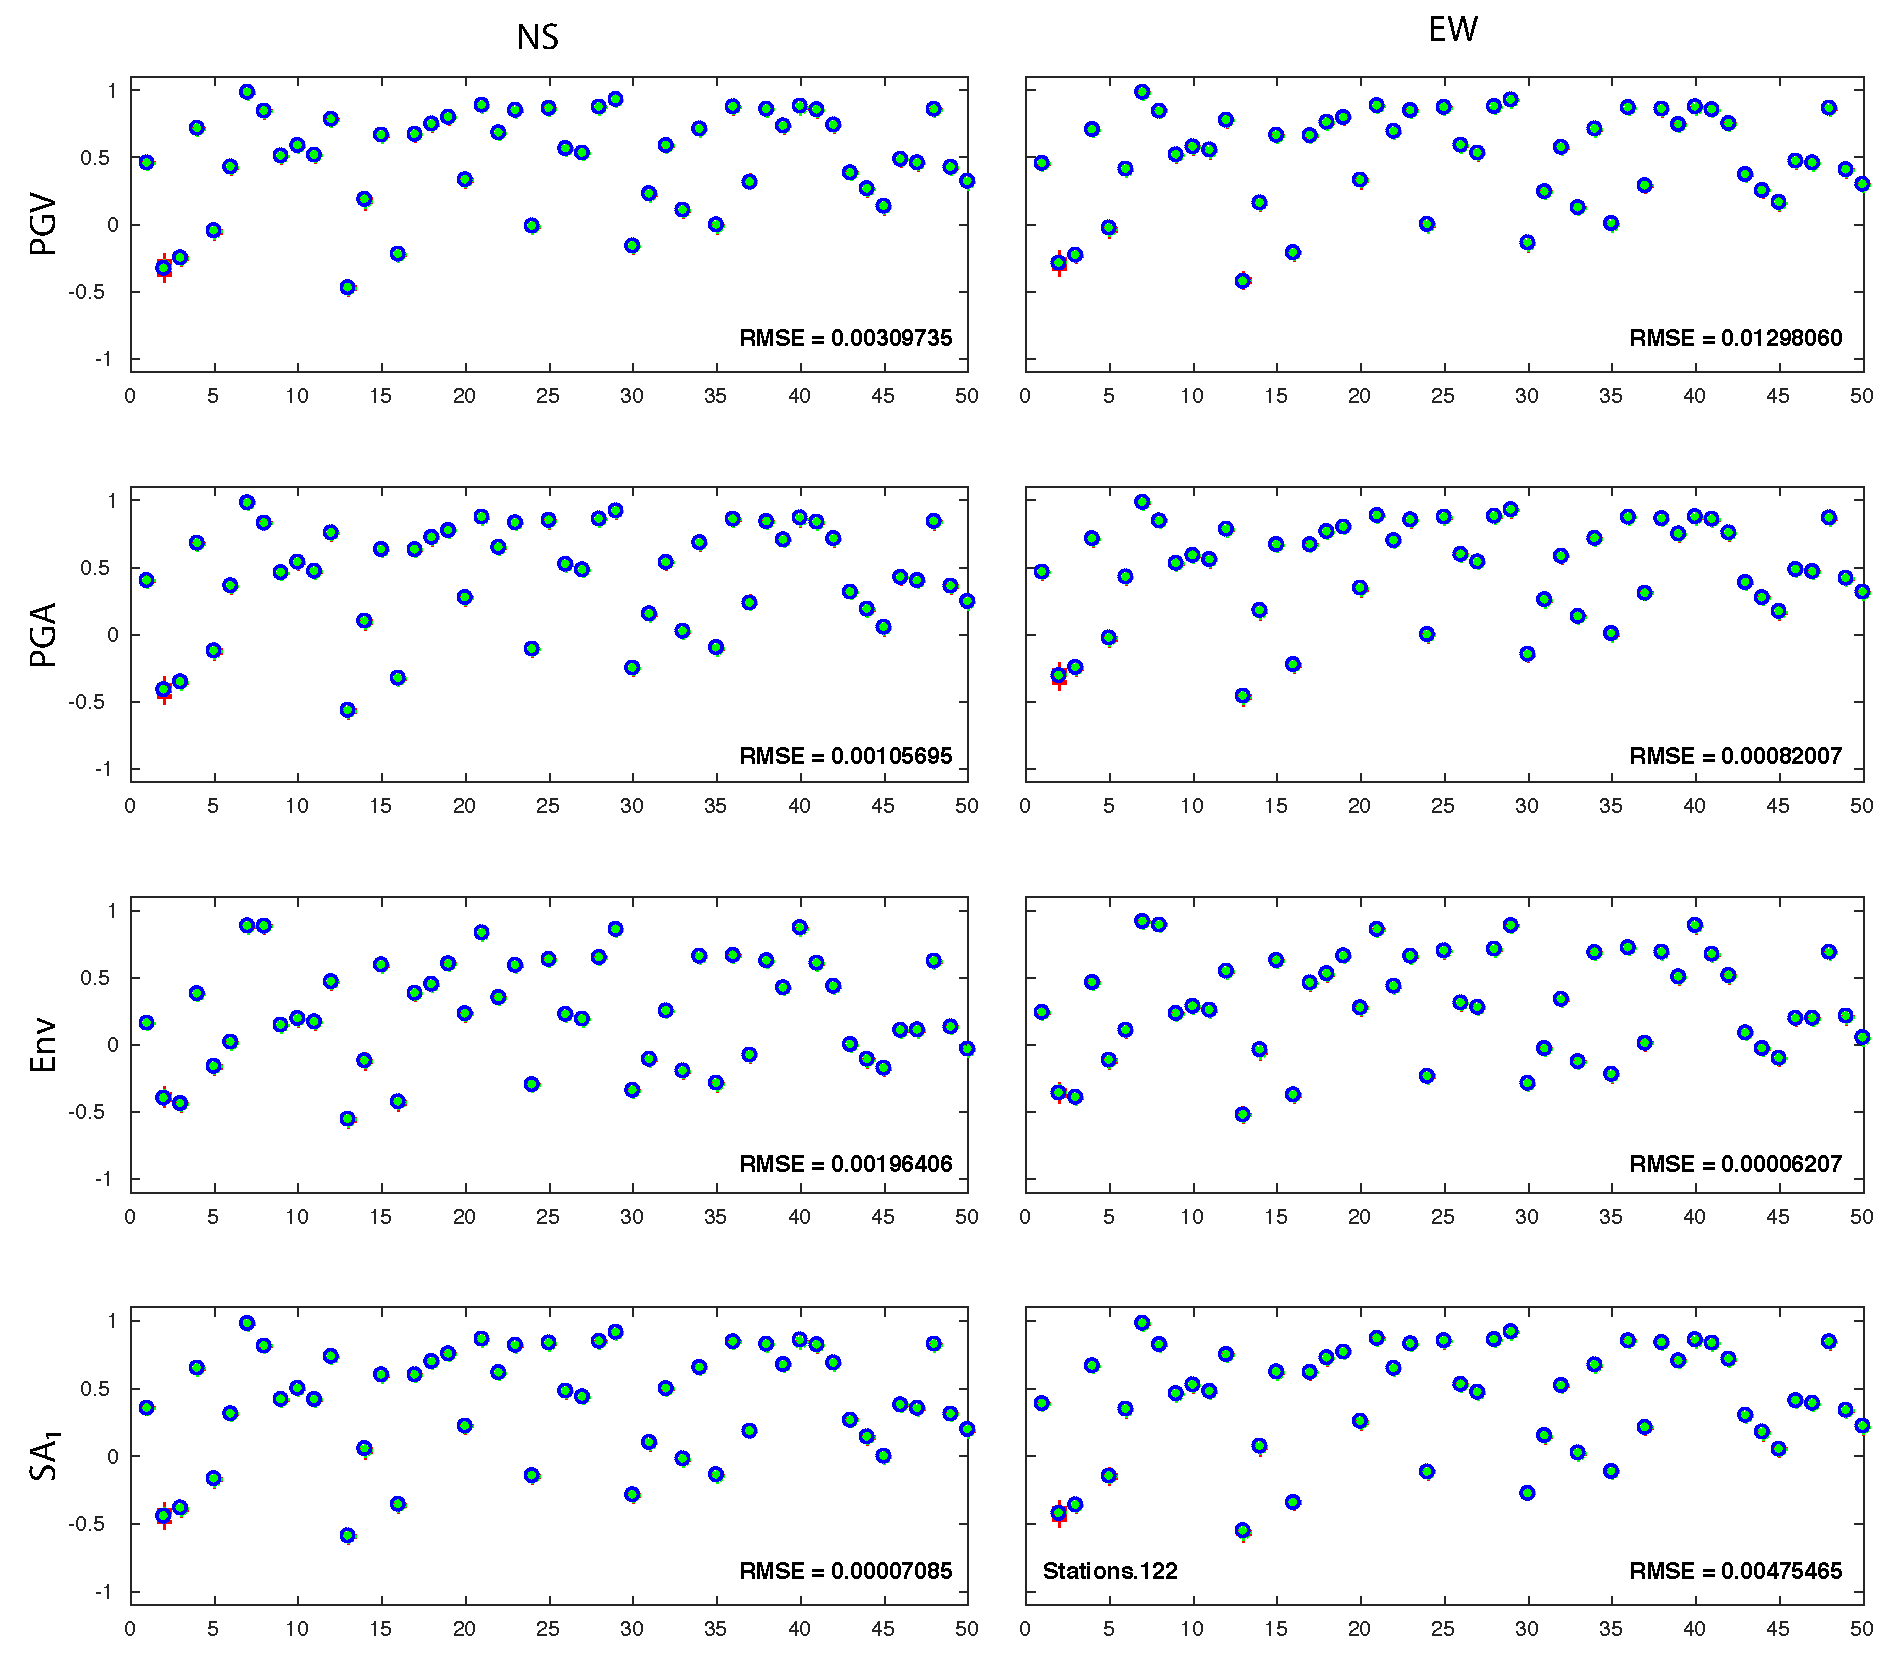
\includegraphics[width=\textwidth]{figures/pdf/Figure_19-st122_het_sim_177.pdf}
    \caption{Accuracy of the results for station number 122 in the heterogenous domain. The station is located in about 42 km from the source (hypo central distance).  }
    \label{fig:ANN_accuracy_stations_122_heterogenous_sim_177}
\end{figure}
 
We follow the steps that we explained at methodology section. We compute the mean of 50 optimized $Q$ values and find the closest $Q$ equation in the training data. We run the optimization process for estimating the new test value which is very close to observation. This process helps us to understand whether the optimization process can find the actual results where we know the input parameters before hand and is very close to the potential field parameters. Those data which pass the following checklist are added to the final Qs-Vs dataset. The criteria is according below:

\begin{itemize}
\item If synthetic solution is converged for a range of shear wave velocity (Standard deviation is an indication of this situation)
\item If the optimizaiotn process successfully locate the input parameters
\end{itemize}

After passing these steps, we generate a dataset and compute another regression analysis to estimate the \qsvs{} relationship that fits the data. As we can see from idealized domains, not all stations and metrics are equally good in extracting all velocity information. This fact also happens in heterogenous domain with fairly complicated source model. Fig.~\ref{fig:used_stations_example} shows four stations that some velocity range of them can pass the defined criteria. 

  \begin{figure}[ht]
    \centering
    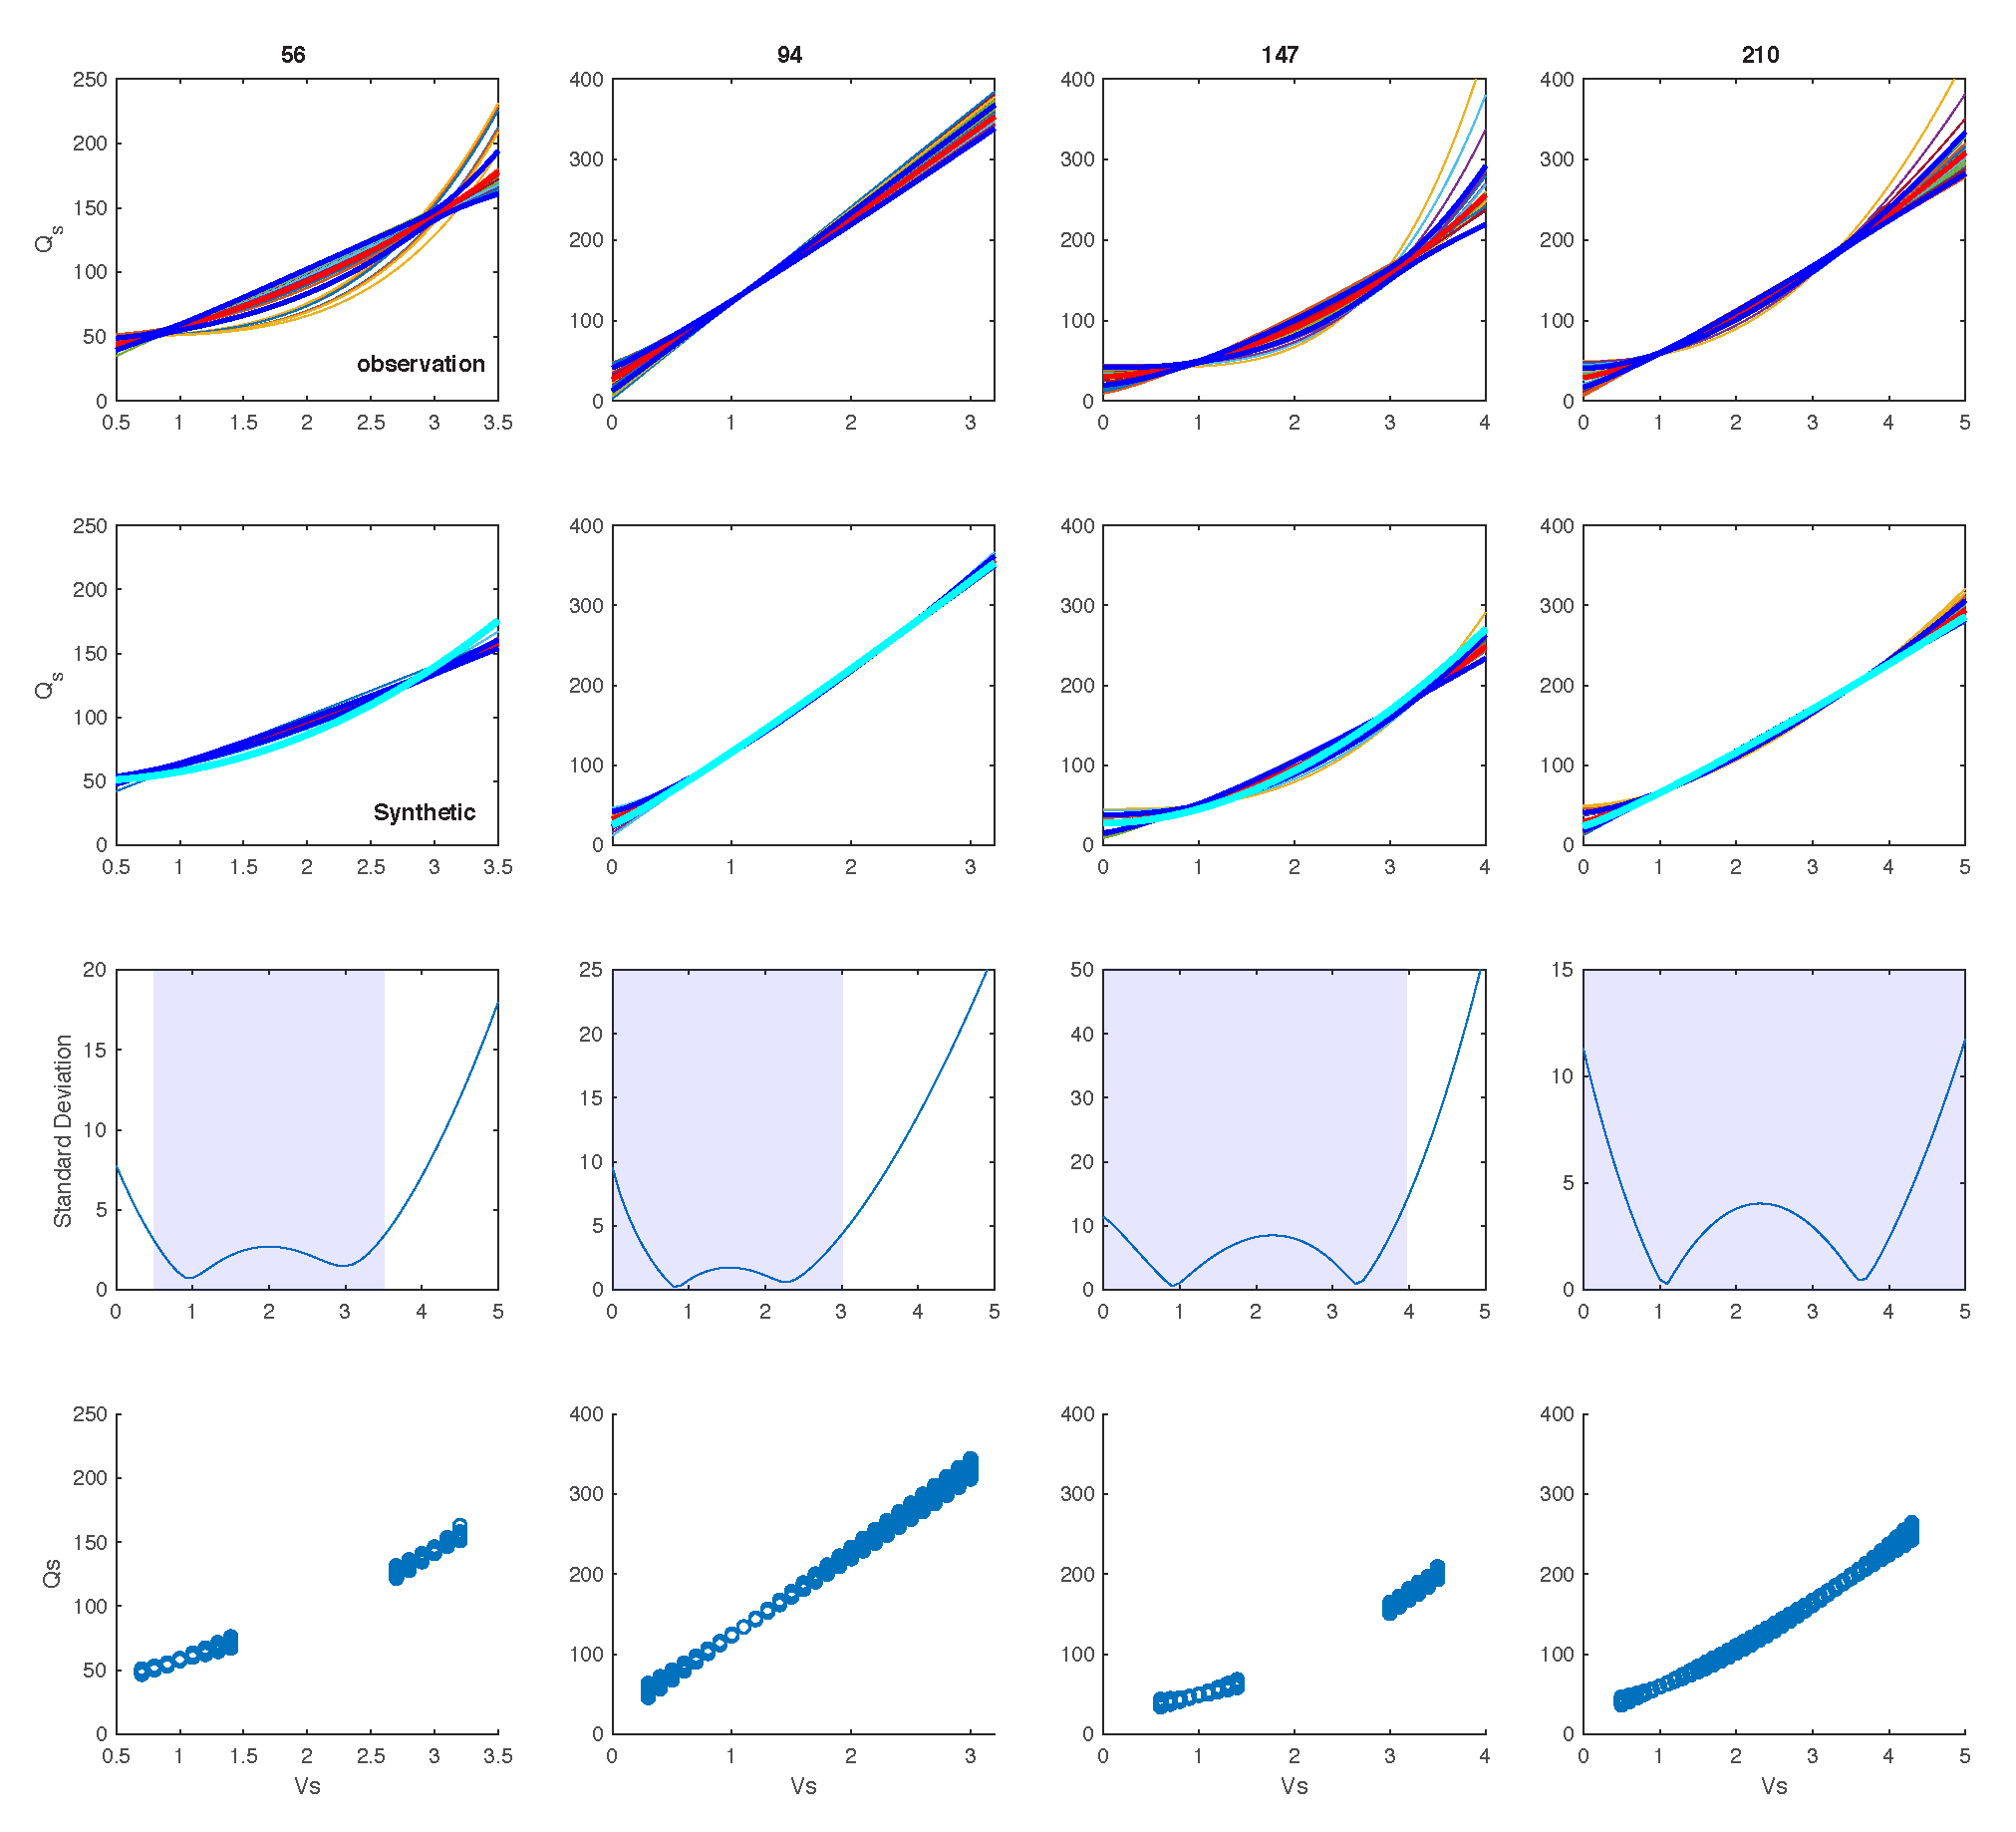
\includegraphics[width=\textwidth]{figures/pdf/Figure_20.pdf}
    \caption{Some of stations in the heterogeneous domain that pass the criteria. The cyan line in synthetic represent the closest available data in training dataset.}
    \label{fig:used_stations_example}
\end{figure}

These four stations are example of stations that part of their shear wave velocity range are used in the final analyses. Each station provides enough information for different range of shear wave velocity. The observation and synthetic are converged at fairly close shear wave velocity ranges for both observation and synthetic. Also in those ranges the algorithm can successfully retrieve the $Q$ value parameters that is used as an input for synthetic target value. The mentioned criteria are met and we can use the results of observation in that range. In order to choose more conservative values for each appropriate shear wave velocity we use only those data that are between $\pm$ standard deviation lines. In all figures these lines are shown using thick blue lines. Similar to the idealized cases, there are stations that cannot pass the defined criteria. Figure.~\ref{fig:unused_stations_example} shows some of these stations. 

  \begin{figure}[ht]
    \centering
    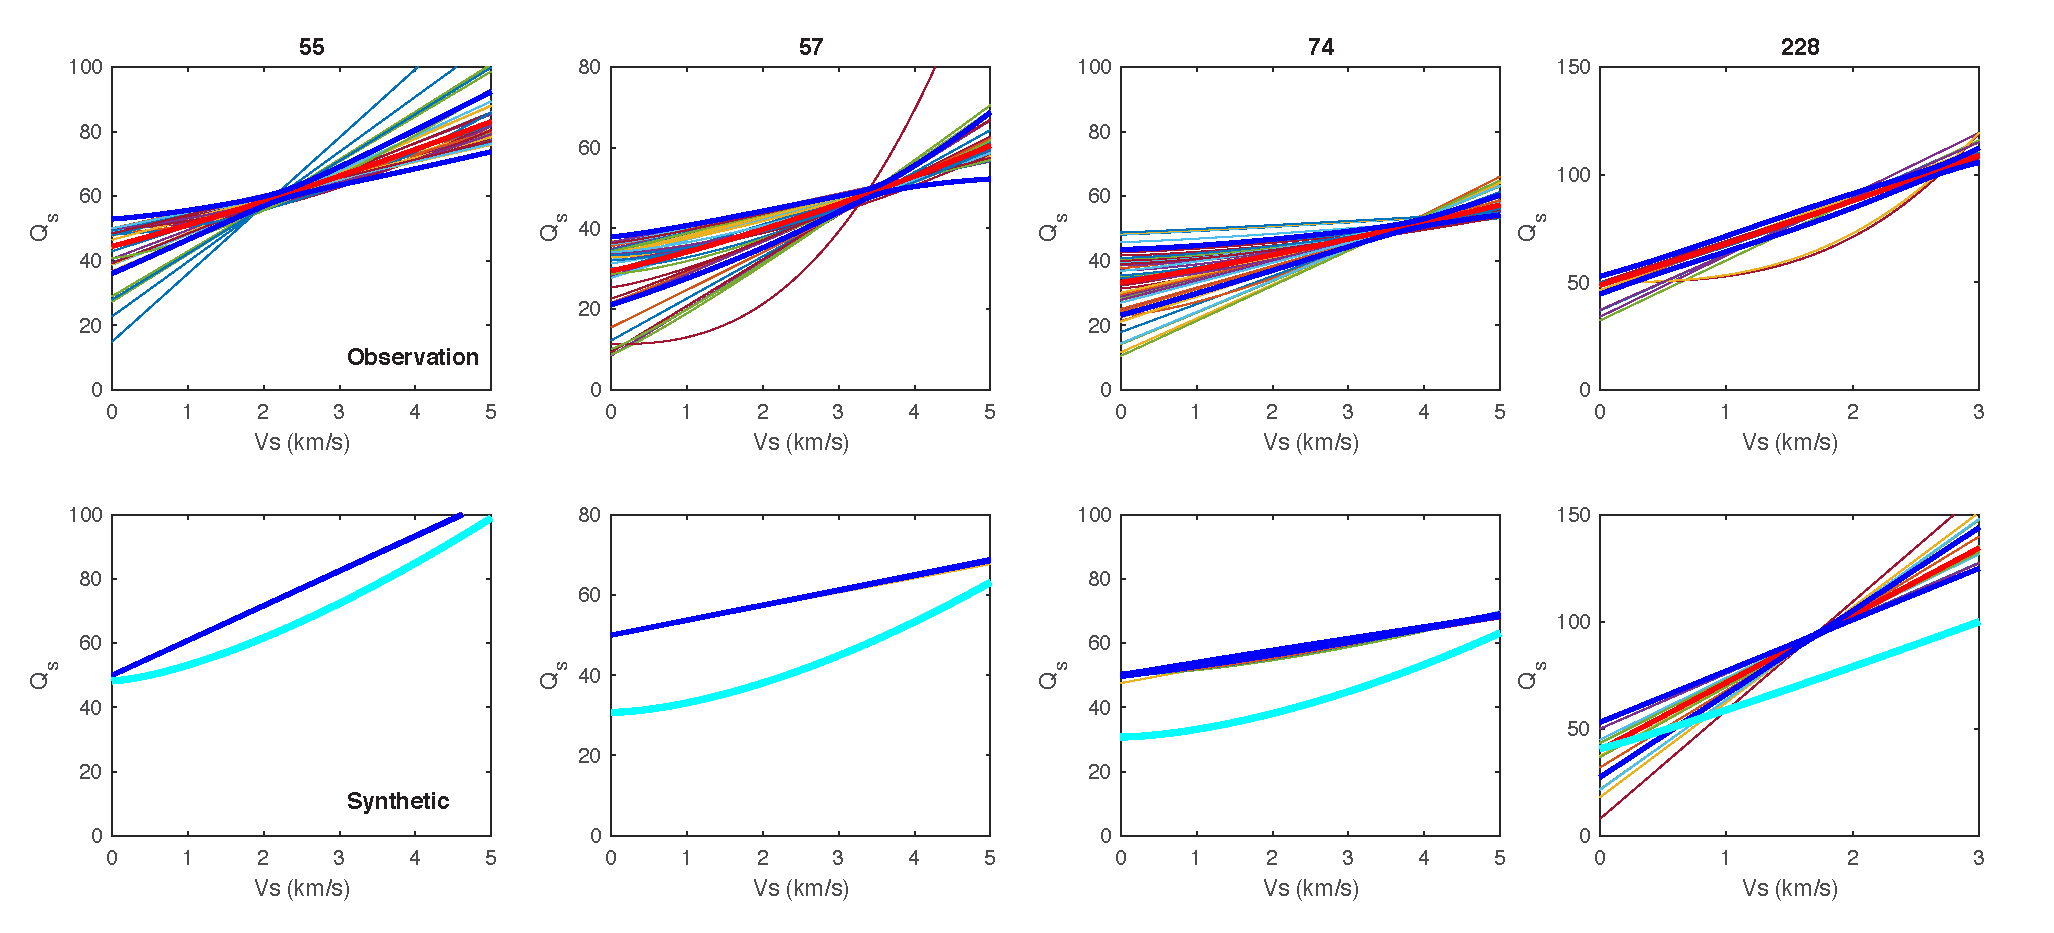
\includegraphics[width=\textwidth]{figures/pdf/Figure_21.pdf}
    \caption{Some of stations in the heterogeneous domain that fails the criteria. }
    \label{fig:unused_stations_example}
\end{figure}

Stations that are represented in Figure.~\ref{fig:unused_stations_example} are not used at the final process. The optimization algorithm provides very converged results at least for three of these stations. However, none of these results are according to the input parameters for target values (dashed green line). This suggests that these stations are not trustable to estimate the observation values. Without the synthetic section of the analyses one arguably can use the converged results of observation. However, the figure shows that the converged $Q$ values are not coincides with initially used $Q$ values. There is a possibility that signal metrics are not conclusive enough to capture the input parameters. The results show that the proposed steps can lead to very accurate and confident parameters. 
The final dataset which we believe is the most appropriate information that we can extract from our dataset in shown in the Fig.~\ref{fig:results_conservative_with_regression} . We use opacity filter and jitter to provide an estimation about the density of points in the figure. In computing the final equation for the Q factor, we ignore data with shear wave velocity less than 350 m/s according to minimum shear wave velocity of the simulations. We use GA optimization to search for the best \qsvs{} relationship that fits dataset.  The final result is $Q_{S}=7.1+60.2 V_{S}^{1.00}$. 


  \begin{figure}[ht]
    \centering
    \includegraphics[width=\textwidth]{figures/pdf/Figure_22.png}
    \caption{Scatter data of stations which passed the optimization criteria. Left: Actual data. Different colors represent different stations. Right: Same data with jitter and opacity filter to represent the data density and distribution.}
    \label{fig:results_conservative_with_regression}
\end{figure}





% The proposed method can retrieve two 

% We can argue that there should not be any problem with optimization process.  

%The idea of effective shear wave velocity or average shear wave velocity is not a novel concept. It is used in many different application to estimate the overall shear wave velocity of a soil profile (e.g., see time average method for shear wave velocity in geotechnical engineering applications).  



%\section{Discussion}

We tested the proposed method on 2008 $Mw$ 5.4 ChinoHills earthquake as a heterogeneous medium with real observation.  The proposed equation is shown in Fig.~\ref{fig:Figure_q_models}  along side the comparison of relationships provided in table. ~\ref{tab:QsVstable}. Notice that the majority of the relationships are independent of depth (z). 

 \begin{figure}
    \centering
    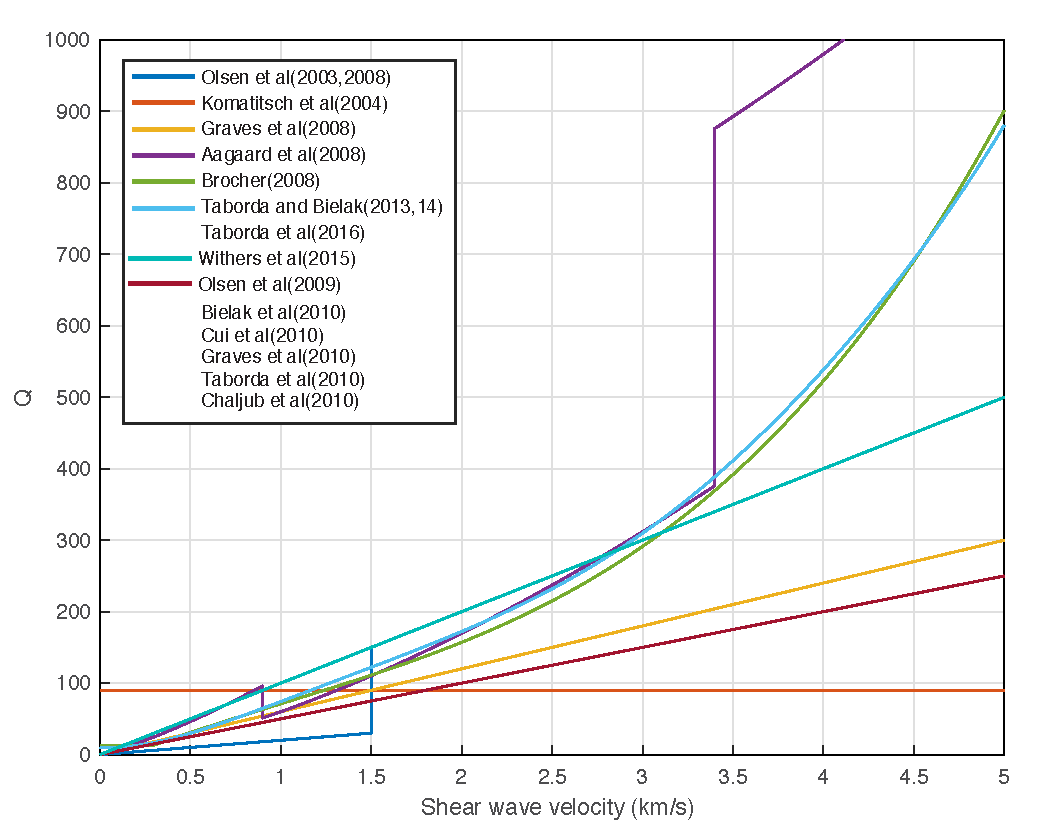
\includegraphics[width=400 px]{figures/pdf/Figure_q_models.pdf}
    \caption{Comparison of Qs rules introduced in table. ~\ref{tab:QsVstable}.}
    \label{fig:Figure_q_models}
\end{figure}

Our proposed relationship---although may not be the definitive one because of limited data used here--- is in agreement with the mean on these values. It is laid between $50Vs$ and $100Vs$ that is commonly used for this region (Lahabra paper, and some other references for 50Vs). Although there is a considerable variation on final dataset shown in Figure.~\ref{fig:results_conservative_with_regression}, the Q equation is not unique for all stations.  Q value is dependent on many other parameters which cause different spatial variation and the end goal is providing a community Q model where all parameters are involved. Variations in QP and QS may be related to porosity, temperature variations, heterogeneity, grain boundary sliding, and lithology. Also, some of the spatial variations in QP and QS appear to be terminated by local fault structure, where on one side of a fault the Q values may be significantly different than on the other \citep{hauksson2006attenuation}.  Moreover, heterogenous domain can cause scattering attention by a redistribution of energy as it is reflected, or converted by small-scale features. These effects may require frequency dependent Q studies \citep{frankel1991mechanisms}.  Also in the near surface sedimentary basin Q is very low \citep{abercrombie1997near}.\\

Therefore, variation of Q values for different stations in a heterogeneous medium are acceptable and predictable. It doubles the importance of the proposed approach where each stations are accurate for different range of parameters. However, for the physics based ground motion simulation in low frequency, it is a common practice to consider Q only as a function of shear wave velocity. Application of proposed method on simplified, layered and heterogenous medium represents its strong potential and robust behavior towards estimating the most accurate parameters for each station.\\

As we discussed earlier, in several stations peak values of signals in observation (mostly PGV and PGA) are higher than without damping simulation. This can happen due to source parameters (e.g., seismic moment, slip function, ...). Therefore, another option for better studying the parameters is including source parameters in the ANNs. This can increase the number of training data, however, will give opportunity of involving more stations in the final model and better constraint the source model. Increasing number of training data in case of higher frequencies will be computationally challenging. In that case, the learning process should take different approach where choose the input values wisely. This will be much more important where one needs to increase the simulation maximum frequency $(f_{max})$.  This concern can be addressed through active learning methods, where different approaches are available toward reducing number of training data, or in other words, eliminating those input data where they most probably will not improve the network \citep[e.g., see][ and the references therein.]{settles.tr09} 



 




%\section{Conclusion}

We present a customized solution approach to study attenuation models through combining machine learning, ground motion simulation, and optimization process used in physics-based ground motion simulation. We train artificial neural networks and ensemble them though bagging approach as a sudo-simulator to estimate the signal parameters based on attenuation model inputs. For each station we estimate the approximate Q value through comparing the results with observation and then we understand at which velocity range the stations, model, and optimization process have the potential of providing accurate results. We test the proposed method on homogenous, layered and heterogenous simulation domains. We applied the proposed solution on several stations of 2008 $Mw$ 5.4 ChinoHills earthquake. The results are in agreement with previous studies. 

We recognize, however, that the proposed equation may not be a definitive one due to use of several stations of one earthquake. In the future follow-up study, it would be ideal to use more signal metrics, more stations and earthquake, as well as include source parameters as an input parameters in sudo-simulators. The procedural steps laid out here, nonetheless, remain valid.    

In summary, we can say that, in physics based ground motion simulation, artificial neural networks can be easily trained for estimating signal metrics. These networks can be used in optimization and uncertainty analysis studies. Example of using these networks with optimization algorithm can provide a dominant/effective shear wave velocity for each seismic station. We also showed that using only peak ground velocity as a signal metric for estimating Q factor parameters may not be enough and adding other parameters improve the results. A combination of machine learning algorithms, optimization process and ground motion simulation can customize the solutions for each individual station and this paper is a successful example of such an application on Q factor parameters studies. 






%
\section{Data and Resources}

Calculations, data processing, and some initial figures were done using MATLAB (\url{http://www.mathworks.com}, last accessed May 2018). Map figures were prepared using the Generic Mapping Tools, GMT (\url{http://gmt.soest.hawaii.edu/}, last accessed May 2018). Additional editing of figures was done using Adobe Illustrator (\url{http://www.adobe.com/Illustrator‎}, last accessed May 2018). The observation data is downloaded from Center for Engineering Strong Motion Data (\url{http://strongmotioncenter.org}, last accessed May 2018)

%
\section{Acknowledgments}
\small

This work was supported by National Science Foundation (NSF) awards: ``SI2-SSI: Community Software for Extreme-Scale Computing in Earthquake System Science'' (ACI-1450451), and ``Improving Earthquake Forecasting and Seismic Hazard Analysis Through Extreme-Scale Simulations'' (OAC-1713792); and Southern California Earthquake Center (SCEC) awards: ``Evaluation of Attenuation Models (Q-Vs Relationships) Used in Physics-Based Ground-Motion Earthquake Simulation through Validation with Data and Comparisons with NGA'' (16-067), and ``Application of Machine Learning in Deterministic Ground Motion Simulation'' (14-022). SCEC is funded by NSF Cooperative Agreement EAR-1600087 and U.S.~Geological Survey Cooperative Agreement G17AC00047. The SCEC contribution number for this paper is xxxx.




\bibliographystyle{spbasic}
\bibliography{references_qpaper_p}


% \section{Introduction}
% \label{sec:introduction}
% Your text comes here. Separate text sections with
% \section{Section title}
% \label{sec:1}
% Text with citations \cite{RefB} and \cite{RefJ}.
% \subsection{Subsection title}
% \label{sec:2}
% as required. Don't forget to give each section
% and subsection a unique label (see Sect.~\ref{sec:1}).
% \paragraph{Paragraph headings} Use paragraph headings as needed.
% \begin{equation}
% a^2+b^2=c^2
% \end{equation}

% % For one-column wide figures use
% \begin{figure}
% % Use the relevant command to insert your figure file.
% % For example, with the graphicx package use
%   \includegraphics{example.eps}
% % figure caption is below the figure
% \caption{Please write your figure caption here}
% \label{fig:1}       % Give a unique label
% \end{figure}
% %
% % For two-column wide figures use
% \begin{figure*}
% % Use the relevant command to insert your figure file.
% % For example, with the graphicx package use
%   \includegraphics[width=0.75\textwidth]{example.eps}
% % figure caption is below the figure
% \caption{Please write your figure caption here}
% \label{fig:2}       % Give a unique label
% \end{figure*}
% %
% % For tables use
% \begin{table}
% % table caption is above the table
% \caption{Please write your table caption here}
% \label{tab:1}       % Give a unique label
% % For LaTeX tables use
% \begin{tabular}{lll}
% \hline\noalign{\smallskip}
% first & second & third  \\
% \noalign{\smallskip}\hline\noalign{\smallskip}
% number & number & number \\
% number & number & number \\
% \noalign{\smallskip}\hline
% \end{tabular}
% \end{table}


%\begin{acknowledgements}
%If you'd like to thank anyone, place your comments here
%and remove the percent signs.
%\end{acknowledgements}

% BibTeX users please use one of
%\bibliographystyle{spbasic}      % basic style, author-year citations
%\bibliographystyle{spmpsci}      % mathematics and physical sciences
%\bibliographystyle{spphys}       % APS-like style for physics
%\bibliography{references}   % name your BibTeX data base


% Non-BibTeX users please use
% \begin{thebibliography}{}
% %
% % and use \bibitem to create references. Consult the Instructions
% % for authors for reference list style.
% %
% \bibitem{RefJ}
% % Format for Journal Reference
% Author, Article title, Journal, Volume, page numbers (year)
% % Format for books
% \bibitem{RefB}
% Author, Book title, page numbers. Publisher, place (year)
% % etc
% \end{thebibliography}

\end{document}

